%
%%%%%%%%%%%%%%%%%%%%%%%%%%%%%%%%%%%%%%%%%%%%%%%%%%%%%%
%                                                    %
%     Modelo para Trabalho de Conclusao de Curso     %
%                                                    %
%                   Template LaTeX                   %
%                                                    %
% Elaboracao  : Grupo PET-Tele                       %
%                                                    %
% Responsaveis:                                      %
%               Marcio Camoleze de Andrade (2008)    %
%               Thiago Muniz de Souza (2008)         %
%                                                    %
% Orientacao  : Prof. Alexandre Santos de la Vega    %
%                                                    %
% Versoes:                                           %
%   - dez/2021 (atualizacao em revisao)              %
%   - set/2017 (primeira revisao estavel)            %
%   - abr/2008 (primeira versao  estavel)            %
%                                                    %
%%%%%%%%%%%%%%%%%%%%%%%%%%%%%%%%%%%%%%%%%%%%%%%%%%%%%%
%

%
\documentclass[12pt,a4paper,oneside]{book}
%
%
%%%%%%%%%%%%%%%%%%%%%%%%%%%%%%%%%%%%%%%%%%%%%%%%%%%%%%
%                Inclusao de pacotes                 %
%%%%%%%%%%%%%%%%%%%%%%%%%%%%%%%%%%%%%%%%%%%%%%%%%%%%%%
%
%
%
%%%%%%%%%%%%%%%%%%%%
%   Pacotes gerais %
%%%%%%%%%%%%%%%%%%%%
%
%
% Padrao brasileiro:
%   a primeira frase eh indentada
%   para todos os paragrafos.
%
\usepackage{indentfirst}
%
%
% Pacotes para lingua portuguesa
%
%%%\usepackage{babel}
%%%\usepackage[brazil]{babel}
\usepackage[brazilian]{babel}
%%%\usepackage[portuguese]{babel}
%%%\babelprovide[import=pt-BR,main]{portuguese}
%
%
%%%\usepackage{ae}
\usepackage{lmodern}
\usepackage[T1]{fontenc}
%
%
% Padrao de codificacao 
% dos caracteres no arquivo '.tex'
%
%%%\usepackage{inputenc}
%\usepackage[ansinew]{inputenc}
\usepackage[utf8]{inputenc}
%
%
% Pacotes matematicos
%
% Package dependency hierarchy 
% in terms of the AMS-LaTeX bundle:
%
% - amsmath (miscellaneous enhancements)
%   - amstext (text embedded in mathematics)
%     - amsgen (*)
%
% - amsbsy (bold symbols)
%   - amsgen (*)
%
% - amsopn (operator name commands)
%   - amsgen (*)
%
% - amssymb (extended symbol collection)
%   - amsfonts (*)
%
% - amsthm (theorem-like environments)
%
% (*) This package has no dependencies.
%
\usepackage{amsmath}
\usepackage{amsfonts}
\usepackage{amssymb}

%
%
% Pacotes graficos
%
%\usepackage{graphics}
\usepackage{graphicx}
\usepackage{subfig}
%\usepackage{subfigure}
\usepackage{epsfig}
%\usepackage{rotating}
%
%
% Pacotes sobre tabelas
%
\usepackage{multirow}
%
%
% Pacote para fazer 'Indice Remissivo'
%
%%%\usepackage{makeidx}
\usepackage{imakeidx}
\makeindex[intoc]
%
%
% Pacotes uteis para revisao do texto
%
% Comentarios de varias linhas
%
\usepackage{comment}
%
%
%%%%%%%%%%%%%%%%%%%%%
% Incluir Códigos   %
%%%%%%%%%%%%%%%%%%%%%
\usepackage{listings}
%
%% Configuracoes do pacote listings
\lstdefinestyle{mystyle}{
language=Python,
basicstyle=\ttm,
% Add keywords here
morekeywords={self, if, True, False, for, except, raise, return, try},
keywordstyle=\ttb\color{deepblue},
% Custom highlighting
emph={set_mode, set_servo_pulsewidth, sleep, OUTPUT, stop, exit},          
% Custom highlighting style
emphstyle=\ttb\color{deepred},    
stringstyle=\color{deepgreen},
% Any extra options here
frame=single,                       
showstringspaces=false,
commentstyle=\color{green}
}
% 
\lstset{
style=mystyle,
breaklines=true
}
%
%
% definicao de comando para Lista de Códigos
%
% Listing -> Código
\renewcommand{\lstlistingname}{Código}
% List of Listings -> Lista de Códigos
\renewcommand{\lstlistlistingname}{Lista de \lstlistingname s}
%
%% PACOTES QUE SERÃO REMOVIDOS APÓS REVISÃO
% Realce de texto
\usepackage{soulutf8}
\usepackage{soul}
% Extensão de letras gregas (Vou tentar Excluir isso)
\usepackage{upgreek}

%%%%%%%%%%%%%%%%% FIM DESSES PACOTES %%%%%%%%%%%%%%

% Marcacao de texto com cor
%
% Explicar...
%
%%%\usepackage{color}
%\usepackage{xcolor}
\usepackage[table,xcdraw]{xcolor}
%
\definecolor{red}  {rgb}{1,0,0}
\definecolor{green}{rgb}{0,1,0}
\definecolor{blue} {rgb}{0,0,1}
\definecolor{deepblue}{rgb}{0,0,0.5}
\definecolor{deepred}{rgb}{0.6,0,0}
\definecolor{deepgreen}{rgb}{0,0.5,0}
\definecolor{green}{rgb}{0,0.8,0}
%
\DeclareFixedFont{\ttb}{T1}{txtt}{bx}{n}{12} % for bold
\DeclareFixedFont{\ttm}{T1}{txtt}{m}{n}{12}  % for normal
%
%
% O pacote 'xurl' 
% faz quebra automatica de linha 
% para um URL muito grande...
%
%%%\usepackage{url}
\usepackage{xurl}
%
\usepackage{hyperref}
%
%
% Explicar e posicionar...
%
%%%\usepackage{memhfixc}
%

%%%%%%%%%%%%%%%%%%%%%%%%%%%%%%%%%%%%%%%%%%%%%%%%%%%%%%
%
%
%%%%%%%%%%%%%%%%%%%%%%%%%%%%%%%%%%%%%%%%%%%%%%%%%%%%%%
%              Formatacao da Pagina                  %
%%%%%%%%%%%%%%%%%%%%%%%%%%%%%%%%%%%%%%%%%%%%%%%%%%%%%%
%
%%%%%%%%%%%%%%%%%%%%%%%%%%%%%%%%%%%%%%%%%%%%%%%%%%%%%%
%              Formatacao da Pagina                  %
%%%%%%%%%%%%%%%%%%%%%%%%%%%%%%%%%%%%%%%%%%%%%%%%%%%%%%

%
% Paper size A4: width=210mm ; height=297mm
%

% horizontal
\setlength{\hoffset}{-1in}

\setlength{\oddsidemargin}{3.0cm} 

\setlength{\textwidth}{160mm}  % (210mm - 30mm - 20mm)

\setlength{\parindent}{1.25cm} % indentacao de cada paragrafo

% vertical
\setlength{\voffset}{-1in}
\addtolength{\voffset}{2.0cm}

\setlength{\topmargin}{0.0cm}

\setlength{\headheight}{5mm}
\setlength{\headsep}{5mm}

\setlength{\textheight}{247mm} % (297mm - 30mm - 20mm)

%%%\setlength{\footskip}{0mm}

%%%%%%%%%%%%%%%%%%%%%%%%%%%%%%%%%%%%%%%%%%%%%%%%%%%%%%
%
%
%%%%%%%%%%%%%%%%%%%%%%%%%%%%%%%%%%%%%%%%%%%%%%%%%%%%%%
%                     Definicoes                     %
%%%%%%%%%%%%%%%%%%%%%%%%%%%%%%%%%%%%%%%%%%%%%%%%%%%%%%
%
% espacamento entre linhas: 
%   \linespread{factor}
%   factor=1.0 (espaço simples)
%   factor=1.3 (espaço 1 1/2)
%   factor=1.6 (espaço duplo)
\linespread{1.3} 
%
\pagestyle{myheadings}
%
\makeindex

%%%%%%%%%%%%%%%%%%%%%%%%%%%%%%%%%%%%%%%%%%%%%%%%%%%%%%


%%%%%%%%%%%%%%%%%%%%%%%%%%%%%%%%%%%%%%%%%%%%%%%%%%%%%%
%             Regras de Divisao Silabica             %
%%%%%%%%%%%%%%%%%%%%%%%%%%%%%%%%%%%%%%%%%%%%%%%%%%%%%%

\hyphenation{tra-ba-lho cur-so En-ge-nhei-ro}

%%%%%%%%%%%%%%%%%%%%%%%%%%%%%%%%%%%%%%%%%%%%%%%%%%%%%%

%
\begin{document}
%

%%%%%%%%%%%%%%%%%%%%%%%%%%%%%%%%%%%%%%%%%%%%%%%%%%%%%%
%                  Capa da Monografia                %
%%%%%%%%%%%%%%%%%%%%%%%%%%%%%%%%%%%%%%%%%%%%%%%%%%%%%%

\begin{titlepage}
  \begin{center}
    \Large{\textsc{Universidade Federal Fluminense} \\
           \textsc{Escola de Engenharia} \\
           \textsc{Curso de Graduação em Engenharia de Telecomunicações} 
          }
    \par\vfill
    \LARGE{Lúcio Folly S. Zebendo\\e\\João Luiz de Amorim Pereira Neto}
    \par\vfill
    \LARGE{Aplica\c{c}\~{o}es de \textit{Drones} em Redes de Computadores: Utilização da plataforma \textit{Raspberry Pi} como computador de bordo.}
    \par\vfill
    \Large{Niterói -- RJ\\
    2022}
  \end{center}
\end{titlepage}

%%%%%%%%%%%%%%%%%%%%%%%%%%%%%%%%%%%%%%%%%%%%%%%%%%%%%%


%%%%%%%%%%%%%%%%%%%%%%%%%%%%%%%%%%%%%%%%%%%%%%%%%%%%%%
%                   Folha de Rosto                   %
%%%%%%%%%%%%%%%%%%%%%%%%%%%%%%%%%%%%%%%%%%%%%%%%%%%%%%

\begin{center}

Lúcio Folly S. Zebendo\\e\\João Luiz de Amorim P. Neto

\vfill

Aplica\c{c}\~{o}es de \textit{Drones} em Redes de Computadores: Utilização da plataforma \textit{Raspberry Pi} como computador de bordo.

\vspace{3.0cm}

\begin{flushright}
\begin{minipage}{0.55\textwidth}
%
Trabalho de Conclusão de Curso 
apresentado ao Curso de Graduação em Engenharia de Telecomunicações 
da Universidade Federal Fluminense, 
como requisito parcial para obtenção 
do Grau de Engenheiro de Telecomunicações. 
%
\end{minipage}
\end{flushright}

\vspace{3.0cm}

Orientador: Prof. Dr. Alexandre Santos de la Vega

Coorientador - Prof. Dr. Lauro Eduardo Kozovits
\vfill

Niterói -- RJ

2022

\end{center}

\pagebreak

%%%%%%%%%%%%%%%%%%%%%%%%%%%%%%%%%%%%%%%%%%%%%%%%%%%%%%


%%%%%%%%%%%%%%%%%%%%%%%%%%%%%%%%%%%%%%%%%%%%%%%%%%%%%%
%                Numeracao em romano                 %
%%%%%%%%%%%%%%%%%%%%%%%%%%%%%%%%%%%%%%%%%%%%%%%%%%%%%%

\pagenumbering{roman}
\setcounter{page}{2}

%%%%%%%%%%%%%%%%%%%%%%%%%%%%%%%%%%%%%%%%%%%%%%%%%%%%%%


%%%%%%%%%%%%%%%%%%%%%%%%%%%%%%%%%%%%%%%%%%%%%%%%%%%%%%%%
%	            Ficha Catalografica                    %
%%%%%%%%%%%%%%%%%%%%%%%%%%%%%%%%%%%%%%%%%%%%%%%%%%%%%%%%

% 
% Info from LaTeX:
%
% \vspace{\fill} in a paragraph will 
%   add the filling vertical space 
%   below the line in which it eventually appears.
%
%   \vspace*{\fill}: the space is never removed.
%
%
% \vfill ends the paragraph at the spot and 
%   adds the filling vertical space.
%

\vspace*{\fill}

  \begin{figure}[!ht]
    \centering
%
% comando para inserir arquivo de imagem
%
%    \includegraphics[width=0.7\textwidth]{FichaCatalografica.jpg}

%
% box inserida apenas para ilustrar posicao da Ficha Catalografica
%
    \framebox{
      \begin{minipage}{0.7\textwidth}
        \centering
        A figura referente ao arquivo 

        \vspace{1cm}
        
        \textit{FichaCatalografica.jpg} 

        \vspace{1cm}
        
        fornecido pela Biblioteca 

        \vspace{1cm}
        
        deverá aparecer aqui. 

        \vspace{1cm}
        
        \textbf{ATENÇÃO: Na versão impressa, 
                essa página deverá ficar 
                no verso da página anterior.}
      \end{minipage}
    } 
  \end{figure}
%
% box inserida apenas para ilustrar posicao da Ficha Catalografica
%

\vspace*{\fill}

\clearpage

%%%%%%%%%%%%%%%%%%%%%%%%%%%%%%%%%%%%%%%%%%%%%%%%%%%%%%


%%%%%%%%%%%%%%%%%%%%%%%%%%%%%%%%%%%%%%%%%%%%%%%%%%%%%%
%                 Folha de Aprovacao                 %
%%%%%%%%%%%%%%%%%%%%%%%%%%%%%%%%%%%%%%%%%%%%%%%%%%%%%%

\begin{center}

Lúcio Folly S. Zebendo\\e\\João Luiz de Amorim P. Neto

\vspace{1.0cm}

Aplica\c{c}\~{o}es de \textit{Drones} em Redes de Computadores: Utilização da plataforma \textit{Raspberry Pi} como computador de bordo.

\vspace{1.0cm}

\begin{flushright}
\begin{minipage}{0.55\textwidth}
%
Trabalho de Conclusão de Curso 
apresentado ao Curso de Graduação em Engenharia de Telecomunicações 
da Universidade Federal Fluminense, 
como requisito parcial para obtenção 
do Grau de Engenheiro de Telecomunicações. 
%
\end{minipage}
\end{flushright}

\vfill

\begin{flushleft}

Aprovada em DIA de MÊS de ANO.

\end{flushleft}

\vfill

BANCA EXAMINADORA

\vfill

\hrulefill \\
Prof. Dr. Alexandre S. de la Vega - Orientador\\
Universidade Federal Fluminense - UFF

\vfill

\hrulefill \\
Prof. Dr. Lauro Eduardo Kozovits - Co-Orientador\\
Universidade Federal Fluminense - UFF

\vfill

\hrulefill \\
Prof. Alexandre S. de la Vega\\
INSTITUIÇÃO

\vfill

\hrulefill \\
Prof. Lauro Eduardo Kozovits\\
INSTITUIÇÃO

\vfill

Niterói -- RJ

2022

\end{center}

\pagebreak

%%%%%%%%%%%%%%%%%%%%%%%%%%%%%%%%%%%%%%%%%%%%%%%%%%%%%%


%%%%%%%%%%%%%%%%%%%%%%%%%%%%%%%%%%%%%%%%%%%%%%%%%%%%
%            Resumo na lingua vernacula            %
%%%%%%%%%%%%%%%%%%%%%%%%%%%%%%%%%%%%%%%%%%%%%%%%%%%%

\chapter*{Resumo}
%
\addcontentsline{toc}{chapter}{Resumo}
%
\thispagestyle{myheadings}
%
Este trabalho é o fruto de um esforço conjunto entre vários discentes e docentes da UFF e iniciativa privada, todos com mútuo 
interesse por VANTs e suas aplicações. O projeto inicial era ideia da Equipe UFFO~\cite{url:equipeuffo} - construir um \textit{drone} 
para vigilância dos campi da UFF. O hardware a ser utilizado era um quadricóptero equipado com um sistema FPV de transmissão analógica. 
Posteriormente, houve-se o interesse de equipar um computador de bordo no \textit{drone} em questão, para fazer aplicações no campo 
da visão computacional com processamento em tempo de voo. Para isso foi utilizado como referência o material da comunidade~\cite{url:ardupilotdoc} 
sobre computadores de bordo~\cite{url:ardupilot-companioncomputers}.\\
%
Para a escolha do computador de bordo foram levados mais em conta fatores de custo e popularidade, com isso a plataforma 
\textit{Raspberry Pi}~\cite{url:raspberrypi} foi a selecionada para esse fim.\\
%
A partir da arquitetura proposta, várias aplicações além da visão computacional são possíveis. Como o computador de bordo em questão 
possui um sistema operacional com propósito geral baseado em \textit{debian}~\cite{url:debian}, além de outras capacidades de Hardware como portas 
\textit{GPIO} para acoplamento de sensores e atuadores e outros barramentos para conexão de periféricos, as possibilidades para esse hardware são muitas.\\
%
Com isso, a aplicação proposta nesse trabalho será a conexão desse computador de bordo à uma rede IP. Várias capacidades da plataforma 
\textit{Raspberry Pi} serão exploradas nos experimentos que sucederão, além disso, serão desenvolvidas aplicações para testar o conceito de 
\textit{Drones} em Redes de computadores.
%

\bigskip

\hl{ Palavras-chave: Raspberry Pi. Drones. VANT. ROS. Equipe UFFO. Robótica. Ardpilot. Pixhawk}

%%%%%%%%%%%%%%%%%%%%%%%%%%%%%%%%%%%%%%%%%%%%%%%%%%%%%%


%%%%%%%%%%%%%%%%%%%%%%%%%%%%%%%%%%%%%%%%%%%%%%%%%%%%%%
%              Resumo na lingua inglesa              %
%                      Abstract                      %
%%%%%%%%%%%%%%%%%%%%%%%%%%%%%%%%%%%%%%%%%%%%%%%%%%%%%%

\chapter*{Abstract}
%
\addcontentsline{toc}{chapter}{Abstract}
%
\thispagestyle{myheadings}
%
This work is a result of a collective effort between some students and teachers from UFF and the private sector, all of them having the mutual interest in UAVs and  their aplications. The first idea of this project was made by UFFO Team~\cite{url:equipeuffo} - to build a drone for surveillance of all UFF campuses. The required hardware would have been a quadcopter equipped with an analog trasmission FPV system. Posteriorly, there was an interest to equip to the same drone an on-board computer, so it could provide some application in computer vision by doing real-time processing, The reference was made by studying the community files~\cite{url:ardupilotdoc} about on-board computers~\cite{url:ardupilot-companioncomputers}.\\
%
The on-board computer was chosen taking into account the cost and popularity, thus, the Raspberry Pi~\cite{url:raspberrypi} was selected for this purpose.\\
%
Based on the proposed architecture, countless features may be implemmented by using its hardware. The on-board computer has an operating system based on debian~\cite{url:debian}, moreover it has numerous GPIO ports that enables the communication to sensors or actuators and also other buses to connect peripherals devices. Hence, there are a plenty possibilities of addons and functionalities.\\ 
%
Therefore, the proposed application of this thesis will be the connection between the on-board computer to an IP network. Many possibilities of Raspberry Pi will be studied and explored in future experiments, besides that, there will be developed some applications to test the concept of drones on a computer network.

\bigskip

\hl{ Keywords: Raspberry Pi. Drones. UAV. ROS. UFFO Team. Robotics. Ardupilot. Pixhawk}

\newpage

%%%%%%%%%%%%%%%%%%%%%%%%%%%%%%%%%%%%%%%%%%%%%%%%%%%%%%


%%%%%%%%%%%%%%%%%%%%%%%%%%%%%%%%%%%%%%%%%%%%%%%%%%%%%%%%
%	                 Dedicatoria                       %
%%%%%%%%%%%%%%%%%%%%%%%%%%%%%%%%%%%%%%%%%%%%%%%%%%%%%%%%

\begin{flushright}
 \begin{minipage}{0.5\textwidth}
  %
  % espaço do topo até o início da dedicatória 
  \vspace{17.0cm} 
  %
  Espaço reservado para a dedicatória.
  %
 \end{minipage}
\end{flushright}



%%%%%%%%%%%%%%%%%%%%%%%%%%%%%%%%%%%%%%%%%%%%%%%%%%%%%%


%%%%%%%%%%%%%%%%%%%%%%%%%%%%%%%%%%%%%%%%%%%%%%%%%%%%%%%%
%	                 Agradecimentos                    %
%%%%%%%%%%%%%%%%%%%%%%%%%%%%%%%%%%%%%%%%%%%%%%%%%%%%%%%%

\chapter*{Agradecimentos}
\addcontentsline{toc}{chapter}{Agradecimentos}

\thispagestyle{myheadings}
%
Agradecemos ao Prof. Alexandre pela orientação durante a nossa estadia no grupo do PET-Tele. Através, 
da nossa participação no grupo foi possível termos um primeiro contato com as plataformas de desenvolvimento 
Arduino e \textit{Raspberry Pi}~\cite{url:raspberrypi}, além de outras atividades que contribuíram para nosso
desenvolvimento acadêmico e profissional.
%
Agradecemos ao Prof. Raul pelo acolhimento na \textit{Equipe UFFO} e pelo incentivo ao estudo e desenvolvimento 
de VANTs. 
%
Agradecemos ao Prof. Lauro Eduardo pelo direcionamento durante a elaboração desse projeto de TCC. 
%
Agradecemos à Equipe UFFO e especialmente ao Raphael Miranda, pelo apoio no desenvolvimento do drone quadcóptero 
utilizado nos experimentos desse trabalho. 
%
Agradecemos à Empresa 6DDrones e especialmente ao Fabio, pelo apoio com infraestrutura e equipamentos para o desenvolvimento 
desse projeto.
%
Agradecemos à comunidade Arducopter pelo grande esforço colaborativo em desenvolver varias das ferramentas utilizadas nesse projeto.
%
Agradeço à Larissa, minha namorada, por todo apoio, carinho e incentivo durante a minha graduação.
%
Agradecemos aos nossos familiares pela cobrança e incentivo nos estudos.
%
%%%%%%%%%%%%%%%%%%%%%%%%%%%%%%%%%%%%%%%%%%%%%%%%%%%%%%


%%%%%%%%%%%%%%%%%%%%%%%%%%%%%%%%%%%%%%%%%%%%%%%%%%%%%%%%
%                   Lista de Figuras                   %
%%%%%%%%%%%%%%%%%%%%%%%%%%%%%%%%%%%%%%%%%%%%%%%%%%%%%%%%
%
\listoffigures
%
\addcontentsline{toc}{chapter}{Lista de Figuras}
%
\thispagestyle{myheadings}
%
%%%%%%%%%%%%%%%%%%%%%%%%%%%%%%%%%%%%%%%%%%%%%%%%%%%%%%


%%%%%%%%%%%%%%%%%%%%%%%%%%%%%%%%%%%%%%%%%%%%%%%%%%%%%%%%
%                   Lista de Tabelas                   %
%%%%%%%%%%%%%%%%%%%%%%%%%%%%%%%%%%%%%%%%%%%%%%%%%%%%%%%%
%
\listoftables
%
\addcontentsline{toc}{chapter}{Lista de Tabelas}
%
\thispagestyle{myheadings}
%
%%%%%%%%%%%%%%%%%%%%%%%%%%%%%%%%%%%%%%%%%%%%%%%%%%%%%%


%%%%%%%%%%%%%%%%%%%%%%%%%%%%%%%%%%%%%%%%%%%%%%%%%%%%%%%%
%                       Sumario                        %
%%%%%%%%%%%%%%%%%%%%%%%%%%%%%%%%%%%%%%%%%%%%%%%%%%%%%%%%
%
\tableofcontents
%
\thispagestyle{myheadings}

\clearpage

%%%%%%%%%%%%%%%%%%%%%%%%%%%%%%%%%%%%%%%%%%%%%%%%%%%%%%


%%%%%%%%%%%%%%%%%%%%%%%%%%%%%%%%%%%%%%%%%%%%%%%%%%%%%%
%                Numeracao em arabico                %
%%%%%%%%%%%%%%%%%%%%%%%%%%%%%%%%%%%%%%%%%%%%%%%%%%%%%%
%
\pagenumbering{arabic}

%%%%%%%%%%%%%%%%%%%%%%%%%%%%%%%%%%%%%%%%%%%%%%%%%%%%%%


%%%%%%%%%%%%%%%%%%%%%%%%%%%%%%%%%%%%%%%%%%%%%%%%%%%%%%%%
%                        Texto                         %
%%%%%%%%%%%%%%%%%%%%%%%%%%%%%%%%%%%%%%%%%%%%%%%%%%%%%%%%
\section{Siglas}

ROS - \textit{Robot Operating System} \\
VANT - Veículo aéreo não tripulado \\
MAVLink - \textit{Micro Air Vehicle Communication Protocol} \\
UART - \textit{Universal asynchronous receiver/transmitter} \\
RXD - \textit{Receive Data}\\
TXD - \textit{Transmit Data}\\

\chapter{Introdução}
%
% retira numeracao da pagina, conforme as normas de apresentacao.
\thispagestyle{empty} 
%
%

Atrelado à popularização da tecnologia, o barateamento dos \textit{drones} tornaram-los capazes de serem usados para além do âmbito militar, ganhando espaço nas industrias cinematográficas, esportivas e do entretenimento, fora para o uso pessoal.

Somado à isso, com o barateamento e miniaturização dos componentes eletrônicos nas últimas décadas, surgiram diversas plataformas eletrônicas de prototipagem, como o Arduíno e também mini computadores como o Raspberry Pi, o que popularizou o estudo das mesmas no âmbito dos drones. 

O uso de mini computadores como o Raspberry Pi já é difundido em aplicações de IOT e robótica e recentemente a comunidade do Ardupilot também explorou e documentou a utilização da plataforma como um computador de bordo, abrindo um leque de possibilidades para as atividades que um VANT (Veículo Aéreo Não Tripulado) pode executar. 

Um computador de bordo permite a utilização de um sistema operacinal completo, e por consequência oferece vários benefícios, como por exemplo capacidades de conexão à rede e a utilização de diversas tecnologias que facilitam o desenvolvimento de drones inteligentes.

Dessa forma, partindo da tecnologia para a utilização de computadores de bordo em drones é possível explorar as capacidades desse sistema conectado à rede. Além disso, é inevitavel a criação de sistemas capazes de realizar o gerenciamento e controle dessas aeronaves através da própria internet, o que será abordado nesse documento.

\section{Motivações}

O sentimento de interesse e empolgação pela tecnologia dos drones dos autores desse texto foram as forças primordiais para a concepção 
do trabalho que se segue. Tal interesse nasceu dentro da Universidade Federal Fluminense através da equipe UFFO~\cite{url:equipeuffo}, 
formada por discentes e docentes da universidade.

Com a experiência adquirida na confecção de um drone quadcóptero simples, descobriu-se a possibilidade de acoplar a este um 
Raspberry Pi~\cite{url:raspberrypi} como computador de bordo da aeronave, expandindo suas capacidades. A partir desta ideia, foram realizados estudos para buscar os métodos e tecnologias mais recentes utilizados nessa configuração de drone. 
Felizmente, muitas dessas tecnologias utilizadas já estavam disponíveis na documentação Open Source do Ardupilot~\cite{url:ardupilotdoc} 
para o equipamento utilizado.

\section{Objetivo}

O primeiro objetivo deste trabalho será o estudo e planejamento da arquitetura do sistema proposto, desde o hardware a ser utilizado, às ferramentas de software e a arquitetura da aplicação que será desenvolvida. 

O segundo objetivo é o desenvolvimento de uma aplicação utilizando as ferramentas e a arquitetura proposta no objetivo anterior. Além disso, o funcionamento do sistema será validado através de um ambiente de simulação. A validação será feita a partir da análise dos resultados.

Por último, com a apuração do sistema, visa-se a construção e configuração de um drone, com as mesmas especificações do usado no segundo objetivo, isso inclui todo o sistema embarcado proposto. Finalmente, serão analisados os resultado obtidos.  

\section{Resultados esperados}

\begin{itemize}
\item Criação de um ambiente de simulação para a validação dos experimentos propostos.
\item Um sistema de controle e navegação para o drone via rede IP.
\item Um drone capaz de realizar comunicação de dados numa rede IP.    
\end{itemize}

\section{Trabalhos correlacionados}

 - Artigos de Drones LTE
 \cite{artigo_relacionado_1}

\section{Organização do documento}

\begin{enumerate}
     \item Introdução teórica 
     
     \begin{enumerate}
     
         \item Definições
         
         Apesar da crescente difusão dos drones na sociedade geral, muitos termos ainda não são conhecidos e devem ser explicados a fim de se compreender a teoria em volta do nosso projeto. Resumidamente, discutiremos os tipos de drones mais comumente comercializados, qual a utilidade de cada parte essencial para um drone operar,  os \textit{softwares} embarcados, o computador de bordo e alguns complementos para aperfeiçoar o projeto.
         
         \item Arquitetura Proposta
 
         Desejamos que, após agregar todas as tecnologias introduzidas, elaborar um sistema composto por uma controladora de \textit{firmware ardupilot} e um computador de bordo capaz de se conectar com uma rede de computadores. O \textit{software} embarcado será desenvolvido utilizando \textit{ROS} e uma \textit{API} será programada em \textit{django} para centralizar a conexão do drone via rede.
 
     \end{enumerate}
     
     \item Metodologia
 
     \item Detalhamento da solução \label{item:solucao}
     
     A nível de \textit{hardware}, para realizar testes iniciais da 
     solução, escolheu-se um drone quadricóptero, a controladora 
     Omnibus f4 pro, um Rapberry Pi, além do \textit{software MavProxy}. 
     Por outro lado, a parte de \textit{software} do projeto, gira em torno
     da conexão entre o pacote \textit{MAVros}, baseado no protocolo 
     \textit{MAVLink}, e o \textit{django framework}.
     
     Em resumo, a
     arquitetura se baseia num modelo cliente-servidor, onde o Rapberry
     é o cliente, e o \textit{django} o servidor, ambos conectados numa mesma
     rede via VPN. Idealmente, outras possíveis soluções seria a conexão de
     um modem LTE (4G) ou NR (5G), o qual permitiria a conexão sem limitações de 
     distância, bastaria estar na área de cobertura do sinal de rede móvel.

     \item Resultados
     
     Estabelecemos com sucesso a conexão entre cliente e servidor. O cliente, composto
     pelo drone, controladora e \textit{Raspberry}, coleta, processa e envia ao servidor os
     dados de telemetria. Já o servidor, formado principalmente pelo \textit{django},
     recebe esses dados e os imprime numa página \textit{web}.



\end{enumerate}




%

\chapter{Introdução teórica}
%
% retira numeracao da pagina, conforme as normas de apresentacao.
\thispagestyle{empty} 
%


\section{Definições iniciais}

\subsection{Drones e VANTs}
Drones são sistemas aéreos automatizados que incluem tanto os VANTs - Veículos Aéreos Não Tripulados, capazes de voar por milhares de 
kilometros, quanto drones pequenos que voam em locais confinados. São veículos aéreos não tripulados, automatizados ou controlados 
remotamente, podem carregar diversos tipos de carga e fazer vários tipos de missões.\\
Devido a avanços nas tecnologias envolvidas na fabricação, nos sistemas de navegação, nos sensores e sistemas de armazenamento de 
energia, uma grande variedade de tipos de drones surgiram nas últimas décadas. 

\subsection{Classificação de VANTs}

\begin{figure}[!htbp]
  \centering
  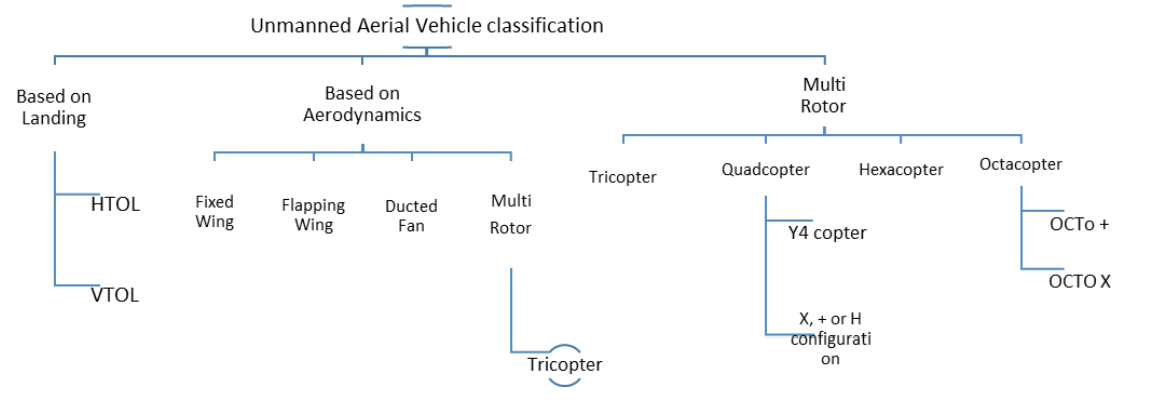
\includegraphics[width=0.7\textwidth]{Images/introducao/drone_classification.png}
  \caption{Classificação de VANTs por tipo de pouso, aerodinâmica e quantidade de rotores.}
  \label{fig:drone_classification.png}
\end{figure}

Como mostrado no organograma da figura a cima~\ref{fig:drone_classification.png}, as categorizações mais comuns para os VANTs são obtidas pelos atributos "tipo de pouso", "aerodinâmica" e "quantidade de rotores".

O tipo de aerodinâmica responsável pela sustentação das aeronaves no ar é bastante diversificado. Uma categoria bem comum de drones são os VANTs de asa fixa, que semelhantemente aos aviões, tiram proveito da geometria das asas e da velocidade gerada por um ou mais motores para obterem sustentação. 

A classificaçao de aterrisagem, com a nomenclatura VTOL e HTOL diz respeito apenas aos VANTs de asa fixa visto que apenas esses tipos de VANTs tiram proveito tanto da aterrisagem vertical quanto da autonomia proveniente do vôo horizontal com asas fixas. 

No presente documento focaremos mais acetuadamente nos drones de asa rotativa, visto que esse tipo de drone será utilizado nos experimentos que sucederão.

\subsection{Componentes dos VANTs de Asa Rotativa}

Os componentes dos drones de asa rotativa variam conforme o tipo de missão. Alguns dos componentes proncipais podem ser listados abaixo:

\begin{enumerate}
  \item Frame
  \item Motores e hélices
  \item Escs
  \item Controladora de voo
  \item Bateria e Placa distribuidora de energia
\end{enumerate}
\subsubsection*{Frame}

O frame de um drone é a base estrutural na qual todos os outros componentes são fixados, ele geralmente é feito de um material leve e 
resistente como fibra de carbono e outros polímeros plásticos. 

\subsubsection*{Bateria e Placa distribuidora de energia}

A bateria é a fonte de energia do drone, geralmente são utilizadas baterias Li-Po (Lítio-Polímero) pela sua boa relação massa/desempenho 
enérgetico, essas baterias possuem uma nomenclatura específica com baase na quantidade de células <explicar melhor as baterias>.

\subsubsection*{Motores e hélices}

Os motores do drone são os responsávei por converter a energia elétrica proveniente das baterias em energia cinética. Geralmente os 
motores utilizados são motores de corrente contínua não escovados (\textit{brushless DC}) <colocar as características físicas desse tipo de motor>.
A partir da corrente elétrica fornecida ao motor ele movimenta a hélice, que devido à sua aerodinamica gera uma força resultante para cima no drone,
a qual é denominada empuxo. 

\subsubsection*{Escs}

Os Escs, ou Eletronic Speed Controlers são os componentes eletrônicos responsáveis por controlar a velocidade dos motores.
Eles são comandados pela controladora de voo, geralmente a partir de sinais PWM <Falar sobre PWM>. Assim como o PWM é utilizado para comandar 
os ESCs, os ESCs utilizam essa modulação para chavear o circuito entre os motores e a bateria controlando assim a velocidade dos motores. 

\subsubsection*{Controladora de Voo}

A controladora de voo é um microcontrolador com software embarcado dedicado às funções básicas da aeronave. Ela possui sensores 
inerciais embutidos para comandar a dinâmica de voo da aeronave, além de possuir interface eletrônica com outros componentes como módulos gps, módulos receptores de rádio, módulos de telemetria entre outros. Sem a controladora de voo, seria uma tarefa humanamente impossível controlar o voo da aeronave, visto que a mesma depende de um feedback contínuo e instantâneo dos parâmetros inerciais. 

\subsection{ArduPilot}
%
\begin{figure}[!htbp]
  \centering
  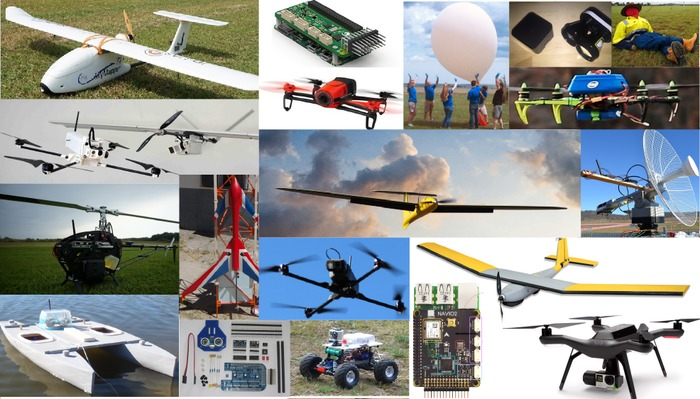
\includegraphics[width=0.7\textwidth]{Images/introducao/ardupilot_vehicles.jpg}
  \caption{Veículos suportados pelo ArduPilot.}
  \label{fig:ardupilot_vehicles.jpg.0}
\end{figure}
%

O ArduPilot é um projeto de código aberto que possui um conjunto de software destinado ao piloto automático de veículos não tripulados, os quais incluem:
\begin{itemize}
  \item Plane - piloto automático para drones de asa fixa.
  \item Copter - piloto automático para drones de asa rotativa.
  \item Rover - piloto automático para veículos terrestres e barcos.
  \item Sub - piloto automático para veículos submarinos.
\end{itemize}

Além de suportar o firmware para todos esses tipos de veículos, a comunidade ArduPilot também se preocupa em desenvolver outras plataformas que auxiliam o desenvolvimento e a utilização do próprio firmware, como por exemplo:

\begin{itemize}
  \item Antenna Tracker - firmware para mirar uma antena automaticamente para o veículo.

  \item Mission Planner - interface de estação de controle em solo escrita em C\# para Windows.
  
  \item APM Planner 2.0 - interface de estação de controle específica para APM escrita em C++ usando os módulos Qt, pode ser executada em Linux, Windows e Mac.
  
  \item MAVProxy - interface de estação de controle em linha de comando ou via script.
  
  \item DroneKit - APM SDK para aplicações executadas de forma embarcada, em mobile, e/ou na nuvem.
  
  \item MinimOSD - visualização de informações de voo em tempo real no visor da interface de FPV.
  \item Tower - interface de estação de controle para celular.  
  \item QGroundControl é uma interface de estação de controle alternativa escrita em C++ usando os modulos Qt.
  \item PX4 - firmware pixhawk para a controladora pixhawk.
  
  \item MAVLink - o protocolo para comunicação entre estação de controle, controladora de voo e alguns componentes incluindo OSD.
  
  \item UAVCAN - protocolo leve e confiável para aplicações de comunicação aeroespacial e robótica, via CAN bus. 
  
\end{itemize}

<LISTAR CONTROLADORAS DE VOO COMPATÍVEIS COM O FIRMWARE>


\subsection{UART}

UART, que vem das palavras \textit{universal asynchronous receive/transmit}, realiza o papel principal na comunicação serial, já que converte os dados entre série e paralelo. Há então uma conversão de paralelo-serial para os dados transmitidos, e uma outra serial-paralelo para os dados recebidos. Existe ainda um \textit{buffer}, cujo objetivo é armazenar dados por tempo limitado em transmissões com alta taxa, sem que haja descarte de dados e consequente perda de informação. Para que não haja fluxo de transmissão caso ambas as partes estiverem prontas, em adição as características citadas, são incorporados circuitos reguladores de fluxo.

A divisão do protocolo é feita em três sub-módulos, gerador de taxa de transmissão, módulo de transmissão e módulo de recepção. O primeiro, se responsabiliza por gerar um sinal de relógio localmente, o qual deve ser muito maior que a taxa de transmissão de dados entre transmissor-receptor. O módulo receptor, por sua vez, recebe os sinais RXD e os converte para dados paralelos. Por fim, o módulo transmissor converte os bytes em bits seriais, com base no padrão de quadro utilizado, e os envia através de sinais TXD. \cite{uart}

\subsection{Telemetria}

A telemetria é uma funcionalidade indispensável nos drones mais modernos, ela permite receber informações dos sensores do drone em tempo real como altitude, velocidade, gps, temperatura, informações da quantidade de carga na bateria dentre outras. Essa transmissão de dados geralmente é feita por um módulo dedicado a isso ou então em módulos receptores de rádio que já possuem essa funcionalidade integrada.

\subsection{Protocolo Mavlink}

MAVLink é um protocolo de comunicação com drones e entre os componentes acoplados ao drone. Essa transmissão consiste no envio de um fluxo de dados, os quais são chamados de tópicos, e escritos em arquivos XML. Dentre as principais vantagens de se utilizar o MAVLink estão a sua eficiência e versatilidade. Em números, a segunda versão do MAVLink tem apenas 14 \textit{bytes} de \textit{overhead} no pacote de comunicação. Além disso, provê métodos de detectar perda de pacotes e dados corrompidos, e garante a autenticação dos pacotes. Outro ponto positivo é o suporte a diversas linguagens, já que o protocolo tem suporte a diferentes tipos de sistemas operacionais e microcontroladores. Por fim, apesar de menos importante para o nosso projeto, vale citar que o protocolo suporta até 255 usuários simultâneos em um mesma rede.
\cite{mavlink}

\subsection{Computadores de Bordo}

Computadores de bordo (ou \textit{Companion Computers}, como são chamados na documentação do ArduPilot) podem ser utilizados para interfacear com o firmware ArduPilot numa controladora de voo através do protocolo MAVLink. Dessa forma, o computador de bordo consegue computar todos os dados MAVLink produzidos pela controladora e com estes pode fazer decisões inteligentes durante o voo. 

Geralmente, no quesito de hardware para esses computadores são escolhidos mini computadores de arquitetura baseada em ARM. Os mini computadores suportados pela comunidade ArduPilot são listados abaixo:

\begin{itemize}
  \item Arduino family
  \item LYCHEE (Cube Carrier Board for Raspberry Pi Compute Module)
  \item NVidia TX1
  \item NVidia TX2
  \item ODroid
  \item Raspberry Pi
\end{itemize}

Já no quesito de software, existem ferramentas, programas e sistemas operacionais específicos para computadores de bordo, tais programas conseguem computar os dados MAVLink vindos da controladora. Alguns dos softwares suportados pela comunidade ArduPilot são listados abaixo:

\begin{itemize}
  \item APSync
  \item DroneKit
  \item FlytOS
  \item Maverick
  \item ROS
  \item Rpanion-server
\end{itemize}


\subsection {Série de computadores Raspberry Pi}
%
O Raspberry Pi é uma série de computadores de placa única e tamanho reduzido, que recebem a denominação  SoC (\textit{System on Chip})~\cite{url:soc} à qual são conectados os seguintes dispositivos: monitor, teclado, e mouse. 

Desenvolvido no Reino Unido pela \href{https://www.raspberrypi.org/}{Raspberry Pi Foundation} tendo, como principais objetivos, contribuir para inclusão digital, promoção de ensino básico em ciência da computação e empoderamento social. Uma alternativa de ensino com baixo custo para escolas e estudantes~\cite{url:raspberry_wiki}. A Tabela~\ref{tab:Especificacoes} apresenta as especificações técnicas do modelo Raspberry Pi Revision 2 - Element 14, utilizado pelo grupo PET-Tele. 
%
\begin{table}[!htbp]
    \centering
    \begin{tabular}{ |c|c| } 
        \hline
        Chip & Broadcom BCM2835 SoC Full HD Processador de Aplicações Multimídia\\
        \hline
        CPU & 700 Mhz ARM1176JZ-F Processador de Baixa Potência de aplicações \\
        \hline
        GPU & Dois Núcleos, VideoCore IV, Co-Processador de Multimídia \\ 
        \hline
        Memória & 512MB SDRAM  \\
        \hline
        Ethernet & Onboard 10/100 Ethernet com conector RJ-45 \\
        \hline
        USB 2.0 & Dois Conectores USB 2.0 \\ 
        \hline
        Saída de Vídeo & HDMI e Composição RCA (PAL e NTSC) \\ 
        \hline
        Saída de Áudio & Conector 3.5 mm ou HDMI \\
        \hline
        Armazenamento & SD, MMC, SDIO Card Slot \\
        \hline
        Dimensões & 8.6 cm X 5.4 cm X 1.7 cm \\ 
        \hline
    \end{tabular}
    \caption{Especificações técnicas do modelo Raspberry Pi Revision 2 - Element14.}
    \label{tab:Especificacoes}
\end{table}

\pagebreak

Na Figura~\ref{fig:rasp3b.jpg.0} é mostrado uma fotografia do modelo. 
Dentre os 25 Pinos presentes neste Raspberry, 17 podem ser usados como entradas ou saídas de uso geral, 5 como terminais comuns (GND), 2 como fontes de tensão de valor +5V e 2 como fontes de tensão de valor +3.3V. 

%
A Tabela~\ref{tab:Raspberry Pinout} reúne uma descrição de todos os pinos.
%
\begin{figure}[!htbp]
    \centering
    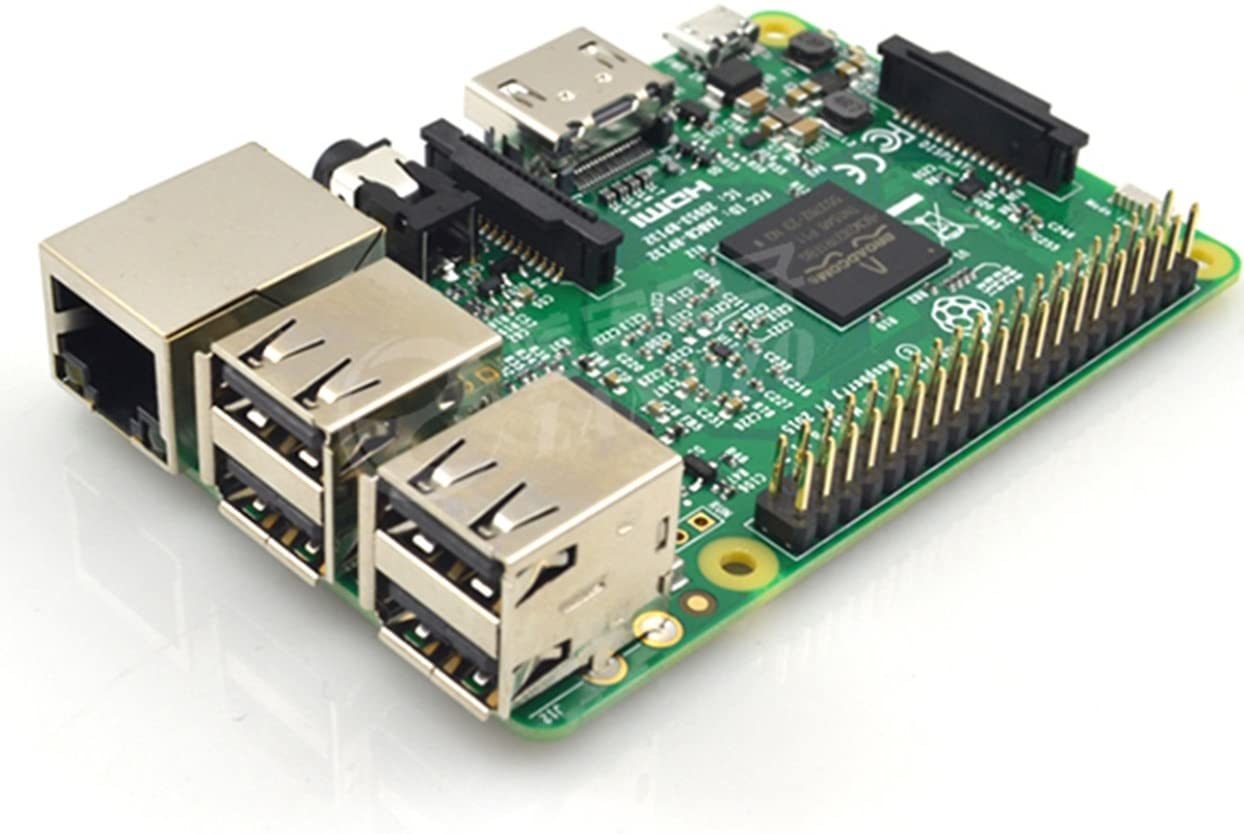
\includegraphics[width=0.7\textwidth]{Images/introducao/rasp3b.jpg}
    \caption{Raspberry Pi Revision 2.0.}
    \label{fig:rasp3b.jpg.0}
\end{figure}
%
\begin{table}[!htbp]
    \centering
    \begin{tabular}{|c|c|c|c|} 
         \hline
         \textbf{N} & \textbf{Descrição} & \textbf{N} & \textbf{Descrição} \\ [0.5ex]
         \hline
         1 & Saída de +3.3V & 14 & Terminal Comum GND\\
         \hline
         2 & Saída de +5V & 15 & GPIO22 \\
         \hline
         3 & GPIO2 | Pull-Up | I2C-SDA & 16 & GPIO23 \\ 
         \hline
         4 & Saída de +5V & 17 & 3V3 \\
         \hline
         5 & GPIO3 | Pull-Up | I2C-SCE & 18 & GPIO24 \\
         \hline
         6 & Terminal Comum GND & 19 & GPIO10 | SPI | MOSI \\ 
         \hline
         7 & GPIO4 & 20 & Terminal Comum GND \\ 
         \hline
         8 & GPIO14 | UART | TXD & 21 & GPIO9 | SPI | MISO\\
         \hline
         9 & Terminal Comum GND & 22 & GPIO25\\
         \hline
         10 & GPIO15 | UART | RXD & 23 & GPIO11 | SPI | CLK\\ 
         \hline
         11 & GPIO17 | UART-RTS & 24 & GPIO8 | SPI | CE0\\
         \hline
         12 & GPIO18 | PWM & 25 & Terminal Comum GND\\ 
         \hline
         13 & GPIO27 & 26 & GPIO7 | SPI | CE1\\ 
         \hline
    \end{tabular}
    \caption{Descrição dos pinos do Raspberry Pi Rev 2.0 - Element 14.}
    \label{tab:Raspberry Pinout}
\end{table}


\subsection{ROS - Robot Operative System}

Robot Operating System, ROS ou ros, é um middleware, 
com foco em robótica, open-source. O ROS não é considerado 
um sistema operacional, mas um conjunto de software 
frameworks para desenvolvimentos de softwares para robôs. 
Oferece serviços a uma vasta gama de computadores, 
como abstração de hardware, controle de dispositivos 
de baixo nível, implementação de funcionalidades usadas 
comumente, troca de mensagens entre processos e 
gerenciamento de pacotes. A arquitetura de grafos 
pode ser usada para representar processos baseados 
em ROS, onde os processos são tidos como vértices, 
os quais podem receber, enviar, e multiplexar 
dados de sensores, controlar, planejar e trocar 
outras mensagens. Apesar da necessidade de baixa latência
e interações rápidas, o ROS não é um \textit{Real-Time
Operating System} (RTOS). Entretanto, embora pouco explorado,
é possível integrar códigos executados em tempo real.
Essa falta de um suporte nativo a códigos de tempo real é
uma preocupação real dos desenvolvedores, os quais planejam 
integrá-los ao ROS 2, projeto que visa ter proveito de 
bibliotecas e tecnologias mais novas. 

As principais bibliotecas do ROS são voltadas para sistemas
Unix, isso se deve ao fato da dependência com diversos
\textit{softwares open-source}. Para essas bibliotecas,
o Ubuntu é listado como "\textit{supported}", entretanto,
para outras distros Linux, como o Fedora, macOS e Windows,
todos são listados como "\textit{experimental}". Ainda assim,
existem exceções, como a biblioteca rosjava, a qual foi 
escrita para Android OS. Apesar disso, oferece uma integração
nativa com o MATLAB, programa que pode ser usado no Linux,
macOS ou Windows. Outro caso a parte é a biblioteca roslibjs,
voltada para desenvolvimento \textit{web} com JavaScript,
que garante compatibilidade com qualquer navegador padrão.


\subsubsection{Mavros}

This package provides communication driver for various autopilots with MAVLink communication protocol. Additional it provides UDP MAVLink bridge for ground control stations (e.g. QGroundControl).

<listar os tópicos>

\subsection{Django}

Django é um \textit{web framework} cuja intenção é tornar o desenvolvimento \textit{web} mais veloz e fácil. Possui uma integração nativa entre banco de dados, \textit{front-end} e \textit{back-end}, apesar de que não seja necessária a utilização de um banco de dados. Primeiramente, podemos citar que todo o esquema do banco é feito através de códigos \textit{python}, pela técnica de mapeamento objeto-relacional, como podemos ver no exemplo a seguir\cite{django}.

\begin{lstlisting}[language=Python]
from django.db import models

class Reporter(models.Model):
    full_name = models.CharField(max_length=70)

    def __str__(self):
        return self.full_name

class Article(models.Model):
    pub_date = models.DateField()
    headline = models.CharField(max_length=200)
    content = models.TextField()
    reporter = models.ForeignKey(Reporter, on_delete=models.CASCADE)

    def __str__(self):
        return self.headline
\end{lstlisting}

No exemplo acima, são instanciadas duas tabelas, \textit{Reporter} e \textit{Article}, e suas respectivas colunas. A fim de criá-las no banco deve-se executar os comandos:

\begin{lstlisting}[language=bash] 
$ python manage.py makemigrations
$ python manage.py migrate
\end{lstlisting}

A partir do momento que os modelos estão criados, podemos registrá-los no arquivo referente ao administrador, o que possibilita a criação, alteração e remoção dos objetos através da \textit{interface web} criada pelo próprio Django. Para habilitar as operações citadas sobre a classe \textit{Article}, por exemplo, basta configurar o arquivo \textit{admin.py} tal como:

\begin{lstlisting}[language=Python]
from django.contrib import admin

from . import models

admin.site.register(models.Article)
\end{lstlisting}

Outro ponto interessante é a possibilidade de configuração de \textit{URLs}. Para isso, devemos criar um código de mapeamento de \textit{URLs} dentro do arquivo \textit{urls.py}, como exemplificado a seguir:

\begin{lstlisting}[language=Python]
from django.urls import path

from . import views

urlpatterns = [
    path('articles/<int:year>/', views.year_archive),
    path('articles/<int:year>/<int:month>/', views.month_archive),
]
\end{lstlisting}



\section{Arquitetura do sistema proposto}

Com todas as tecnologias devidamente estudadas, deseja-se criar um sistema composto pelas mesmas e explorar as capacidades de tal sistema. Para isso, utilizaremos um drone com controladora de firmware ArduPilot e um computador de bordo capaz de se conectar com uma rede de computadores. O software embarcado será desenvolvido utilizando ROS e uma API será desenvolvida em Django para se comunicar com o drone via rede. 
%    \centering
%    \includegraphics{Images/introducao/planta_inicial.png}
%    \caption{Diagrama em blocos da planta didática em configuração original.}
%    \label{fig:planta_inicial}
%\end{figure}


%%%%%%%%%%%%%%%%%%%%%%%%%%%%%%%%
%%%%%%%% Metodologia %%%%%%%%%%%
%%%%%%%%%%%%%%%%%%%%%%%%%%%%%%%%

\chapter{Metodologia}
\label{chapter:Metodologia}
%
% retira numeracao da pagina, conforme as normas de apresentacao.
\thispagestyle{empty} 
%
\section{Pesquisa}
%
\section{Objetivos do método aplicado}
A metodologia aplicada possui objetivo descritivo e exploratório. Após a realização de cada etapa do projeto serão feitos experimentos para comprovar o devido funcionamento do sistema e para este serão comentadas as possibilidades de aplicações.

\section{Abordagem}
Adotar-se-á uma análise qualitativa dos resultados obtidos a partir da implementação do novo sistema, em observância aos seguintes questionamentos:
\begin{enumerate}
    \item Com o sistema desenvolvido será possível receber dados de telemetria via rede?
    \item Com o sistema desenvolvido será possível ao operador do sistema, controlar o drone remotamente?
    \item O quão seguro é o sistema desenvolvido? Quais riscos de segurança estão submetidos a tal sistema?
    \item pergunta avaliativa 3
    \item pergunta avaliativa 4
\end{enumerate}
%
%%%%%%%%%%%%%%%%
%

\section{Descrição do problema}
De forma resumida, deseja-se, a partir de um drone montado com todos os seus componentes essenciais, acoplar um Raspberry Pi à controladora do mesmo para conectar o conjunto à rede de computadores e com isso expandir suas capacidades. Algumas questões surgem quanto a esse projeto, como por exemplo: Qual arquitetura de software a ser utilizada, ou seja como o software a ser desenvolvido será organizado? Qual arquitetura de rede a ser utilizada, por exemplo, par-a-par ou cliente-servidor? No quesito de comunicação na internet, na qual muitas vezes não se tem o controle da rede, como seria feita essa comunicação?

%%%%%%%%%%%%%%%%%%%%%%%%%%%%%%%%%%%%%%%%%%%%%%%%%%%%%%%
%
\chapter{Detalhamento da solução}
%
% retira numeracao da pagina, conforme as normas de apresentacao.
\thispagestyle{empty} 
%

\section{Ambiente de simulação}
%
\begin{figure}[!htbp]
  \centering
  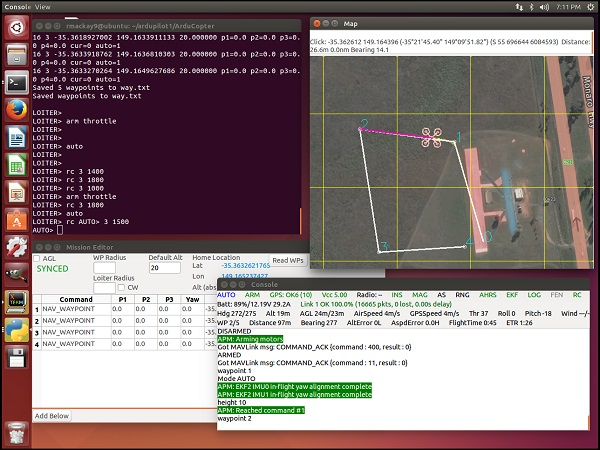
\includegraphics[width=0.7\textwidth]{Images/Desenvolvimento/sitl_demo.jpg}
  \caption{Demonstração do Software In The Loop.}
  \label{fig:sitl_demo.jpg.0}
\end{figure}
%

O projeto ArduPilot possui um rico conjunto de ferramentas que auxiliam no desenvolvimento de aplicações para drones. O próprio código fonte do firmware ArduPilot pode ser compilado e carregado em um ambiente de simulação. O executável responsável por isso é chamado SITL (Software In The Loop), cujo digrama é apresentado na figura \ref{fig:sitl_arq.jpg.0}, esse programa consegue integrar-se com outros formando um ambiente de simulação completo. O MavProxy é utilizado para fazer a interface de comunicação entre o operador e a controladora em ambiente simulado. Além disso, é possível integrar com um simulador de física e dessa forma simular a dinâmica de voo da aeronave. A simulação da dinâmica de voo da aeronave geralmente vem acompanhada com a integração de algum software de visualização como no caso do Flight Gear e do Gazebo, o qual estaremos utilizando. A integração de todos esses componentes no ambiente de simulação forma um loop, e com isso temos o nome Software In The Loop. Essa aplicação é essencial para o desenvolvimento pois permite a execução do ArduPilot sem a utilizaçao de nenhum hardware.

%
\begin{figure}[H]
  \centering
  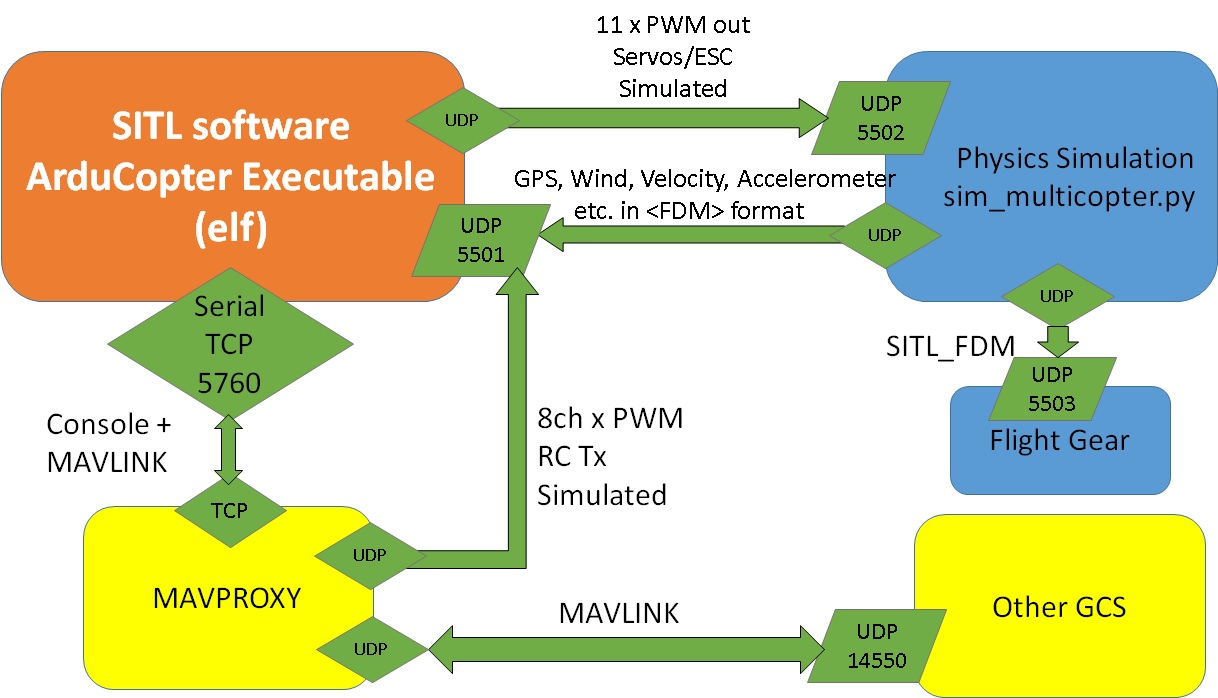
\includegraphics[width=0.7\textwidth]{Images/Diagramas/sitl_arq.jpg}
  \caption{Arquitetura do Software In The Loop}
  \label{fig:sitl_arq.jpg.0}
\end{figure}
%



A inicialização do SITL é feita utilizando o script python demonstrado na figura \ref{fig:sim_vehicle.png.0}, que é disponibilizado junto ao código fonte do ArduPilot no seu repositorio do github.

%
\begin{figure}[H]
  \centering
  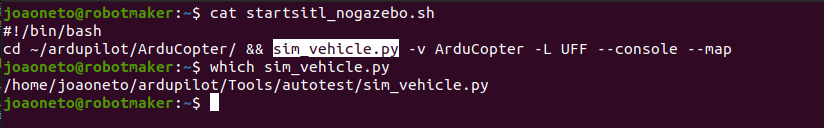
\includegraphics[width=0.7\textwidth]{Images/Desenvolvimento/sim_vehicle.png}
  \caption{sim\_vehicle.py}
  \label{fig:sim_vehicle.png.0}
\end{figure}
%

Como demonstrado na figura \ref{fig:sim_vehicle.png.0} criamos um script bash para executar o ambiente de simulação, nos parametros especificamos que queremos simular o firmware ArduCopter, utilizando as interfaces de mapa e console. Além disso, inserimos como parametro a localização em coordenadas do campo de futebol da UFF no Campus de Gragoatá. O resultado da execução desse script pode ser visualisado na figura \ref{fig:startsitl_nogazebo.png.0}.

%
\begin{figure}[H]
  \centering
  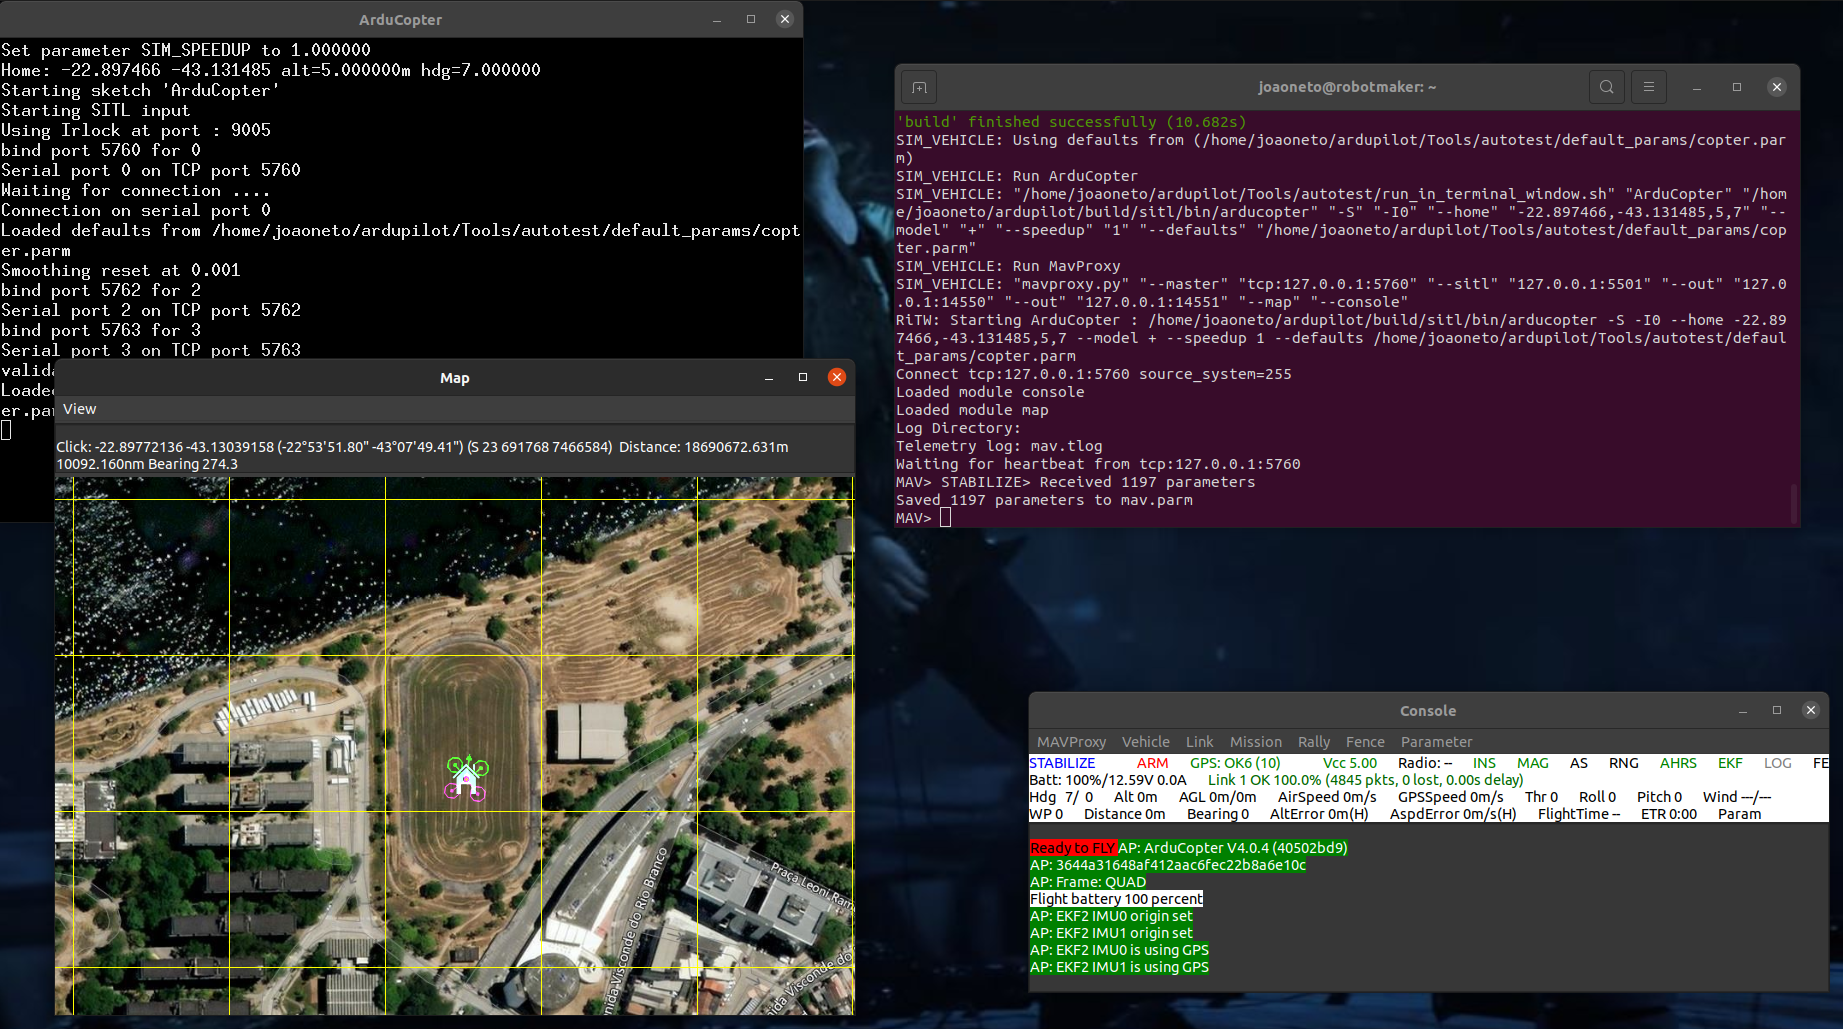
\includegraphics[width=0.8\textwidth]{Images/Desenvolvimento/startsitl_nogazebo.png}
  \caption{startsitl\_nogazebo.sh}
  \label{fig:startsitl_nogazebo.png.0}
\end{figure}
%

Fizemos também um segundo script bash com os parametros necessários para a conexão com o Gazebo, que é o software que simula um mundo em 3D para o drone. Separamos nesses dois scripts, pois na maioria das vezes a simulação em 3D nao é necessária e consome muito dos recursos da máquina que a executa.

%
\begin{figure}[H]
  \centering
  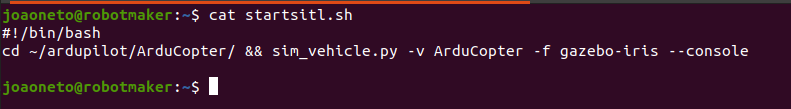
\includegraphics[width=0.8\textwidth]{Images/Desenvolvimento/startsitl.sh.png}
  \caption{startsitl.sh com Gazebo}
  \label{fig:startsitl_nogazebo.png.0}
\end{figure}
%

O modelo de mundo 3D utilizado no Gazebo para a integração com o SITL foi obtido a partir do repositorio de un canal do \textit{Youtube} chamado \cite{url:iq}. 
%
\begin{figure}[H]
  \centering
  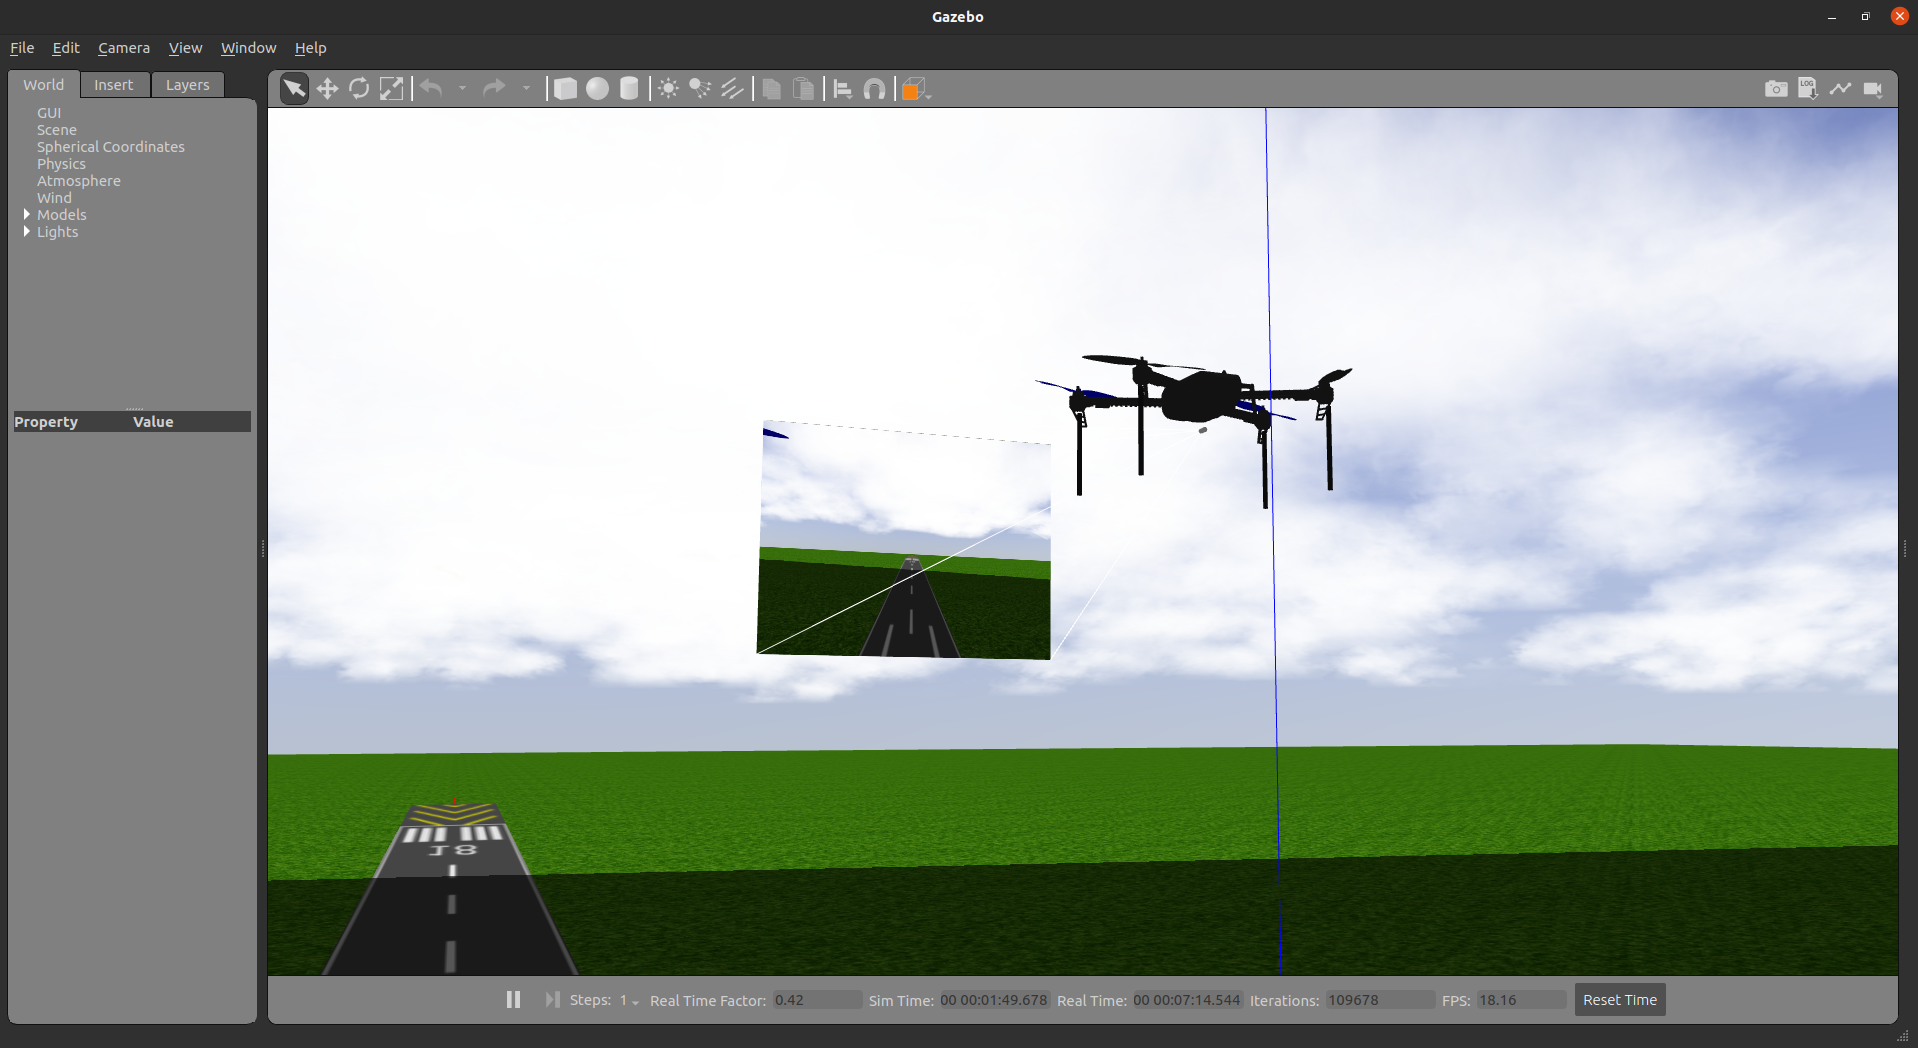
\includegraphics[width=0.7\textwidth]{Images/Desenvolvimento/sitl_gazebo.png}
  \caption{Software In The Loop com Gazebo}
  \label{fig:sitl_gazebo.png.0}
\end{figure}
%
Essa instancia do Gazebo é iniciada a partir de um nó do ROS, que é executado com o comando da figura \ref{fig:ros_gazebo.png.0}.
%
\begin{figure}[H]
  \centering
  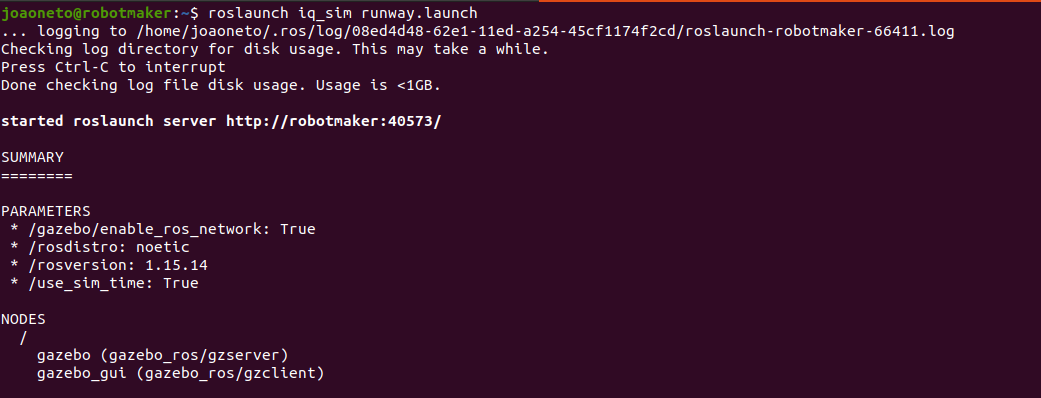
\includegraphics[width=0.7\textwidth]{Images/Desenvolvimento/ros_gazebo.png}
  \caption{Nó do Gazebo - ROS}
  \label{fig:ros_gazebo.png.0}
\end{figure}
%

Com isso, obtemos um ambiente de teste de desenvolvimento para as aplicações que sucederão. Os benefícios de se utilizar um ambiente de simulaçao como este é que não colocamos em risco o equipamento de hardware, nem as pessoas que seriam envolvidas em testes de campo. Além disso, o teste no ambiente computacional se torna mais prático, descartando toda a logística necessária para se deslocar com todo o equipamento para um campo aberto e com baixa densidade populacional.

O processo de instalação do ambiente de desenvolvimento do ArduPilot está bem documentado nos appendices deste documento, nesse processo também está incluído a instalação de dependencias para executar o ambiente de simulação. 

\section{Ambiente de Simulação com o Mavros}

O Mavros como dito na parte introdutória, é um nó de ROS que publica e subscreve dados da controladora de voo, essas mensagens são trocadas utilizando o protocolo MAVLink. O Mavros é geralmente configurado para realizar a comunicação através de um dispositivo serial, que no linux é identificado por um arquivo no diretório /dev. Entretanto, para fazer o Mavros se comunicar com o SITL, deve-se fazer uma modificação no arquivo de inicialização, arquivo com extensão \textit{.launch} no diretório launch do pacote.

No diretório launch do pacote são observados vários arquivos \textit{.launch} utilizados para iniciar o nó do Mavros com diferentes parâmetros. O apm.launch foi modificado como indicado na figura \ref{fig:mavros_launch.png.0}, para utilizar a porta de rede específica do MavProxy no SITL e não o dispositivo serial, comentado na linha superior.
%
\begin{figure}[H]
  \centering
  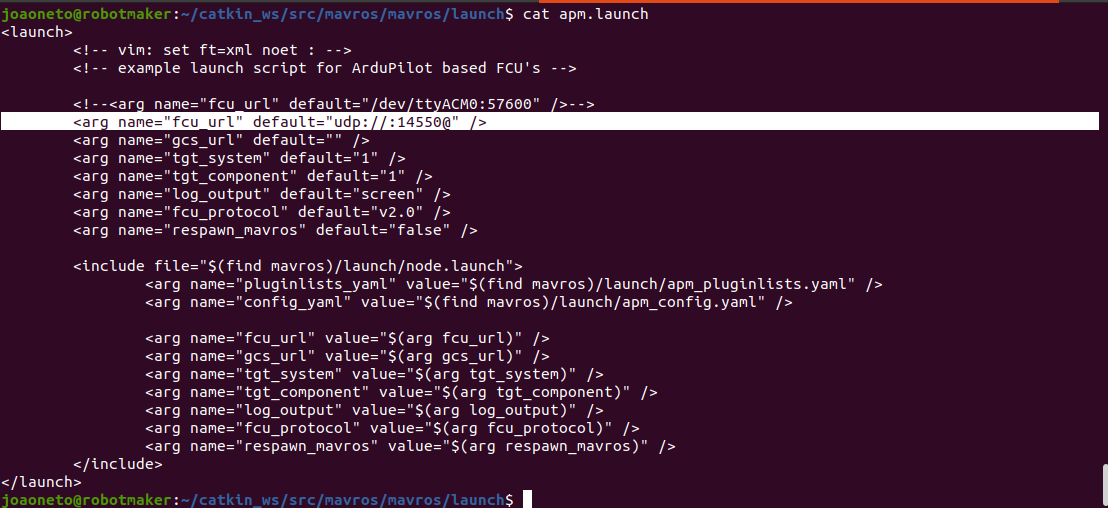
\includegraphics[width=0.7\textwidth]{Images/Desenvolvimento/mavros_launch.png}
  \caption{apm.launch do Pacote Mavros}
  \label{fig:mavros_launch.png.0}
\end{figure}
%
Com essa modificação, o nó do Mavros pode ser iniciado normalmente em conjunto com o SITL e é possível subscrever e publicar mensagens MAVLink nos tópicos para a controladora de voo no ambiente simulado. 
%
\begin{figure}[H]
  \centering
  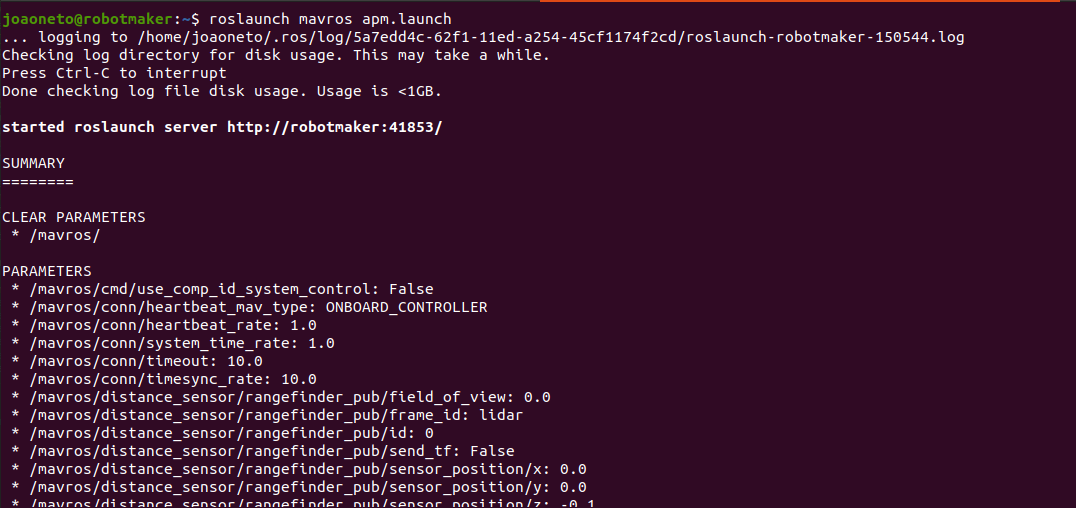
\includegraphics[width=0.7\textwidth]{Images/Desenvolvimento/mavros_execution.png}
  \caption{Execução do Mavros}
  \label{fig:mavros_execution.png.0}
\end{figure}
%
Alguns dos tópicos providos pelo Mavros são listados pelo comando rostopic list na figura \ref{fig:mavros_rostopic_list.png.0}. 
%
\begin{figure}[H]
  \centering
  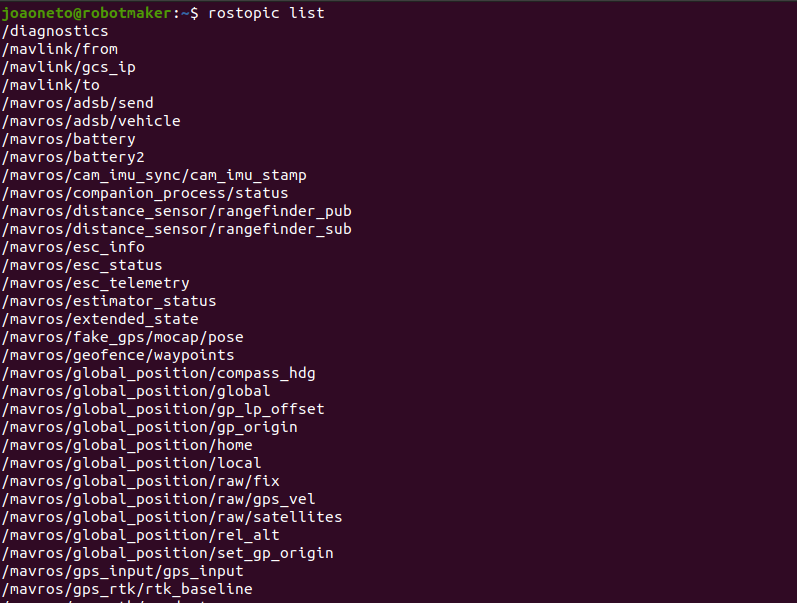
\includegraphics[width=0.7\textwidth]{Images/Desenvolvimento/mavros_rostopic_list.png}
  \caption{Tópicos do Mavros}
  \label{fig:mavros_rostopic_list.png.0}
\end{figure}
%
Por exemplo, o tópico correspondente a localização GPS da controladora de voo é o global\_position. É possível subscrever e acompanhar as mensagens que chegam da controladora nesse tópico pelo comando da figura \ref{fig:mavros_rostopic_echo.png.0}.
%
\begin{figure}[H]
  \centering
  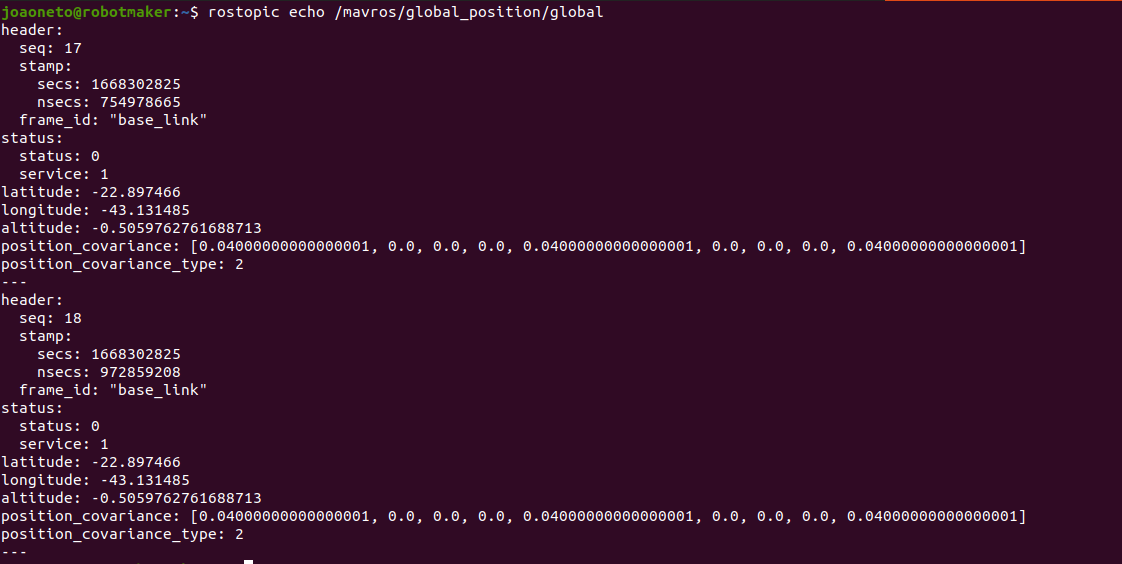
\includegraphics[width=0.7\textwidth]{Images/Desenvolvimento/mavros_rostopic_echo.png}
  \caption{Tópicos do Mavros}
  \label{fig:mavros_rostopic_echo.png.0}
\end{figure}
%

Os tópicos do ROS são fácilmente acessados através de linguagens de programação como C++ e Python. Em particular esta última, possui um módulo chamado rospy que permite a criação de aplicações do ROS, com este módulo é possível desenvolver nós inteiramente usando Python. Agora que temos o Mavros agindo como interface da aeronave, é possível desenvolver o software embarcado que também será um nó, ele irá se comunicar com o Mavros e com a aplicação em Django que será desenvolvida.

\section{Arquitetura da aplicação}

<mostrar diagrama estrutural>

\begin{enumerate}
  \item mavros 
  \item iq\_gnc
  \item drone\_telemetry\_over\_network
  \item drone\_control\_over\_network
  \item Drone\_CCS\_API (Cloud Control Station)
\end{enumerate}

\section{Arquitetura da aplicação de rede}

Modelo cliente servidor, no qual o raspberry e o servidor da API estão numa mesma VPN. 

\section{Outras arquiteturas possíveis para o sistema proposto}

LTE e 5G.

\section{Primeiros testes com o drone quadricóptero}

De posse de um drone quadricóptero com a controladora de voo Omnibus f4 pro, foram estabelecidos os primeiros testes de conexão entre o Raspberry Pi e o firmware ArduPilot. O diagrama de montagem do equipamento foi o seguinte:

\subsection{Diagrama de conexão dos componentes de hardware}
%
\begin{figure}[!htbp]
  \centering
  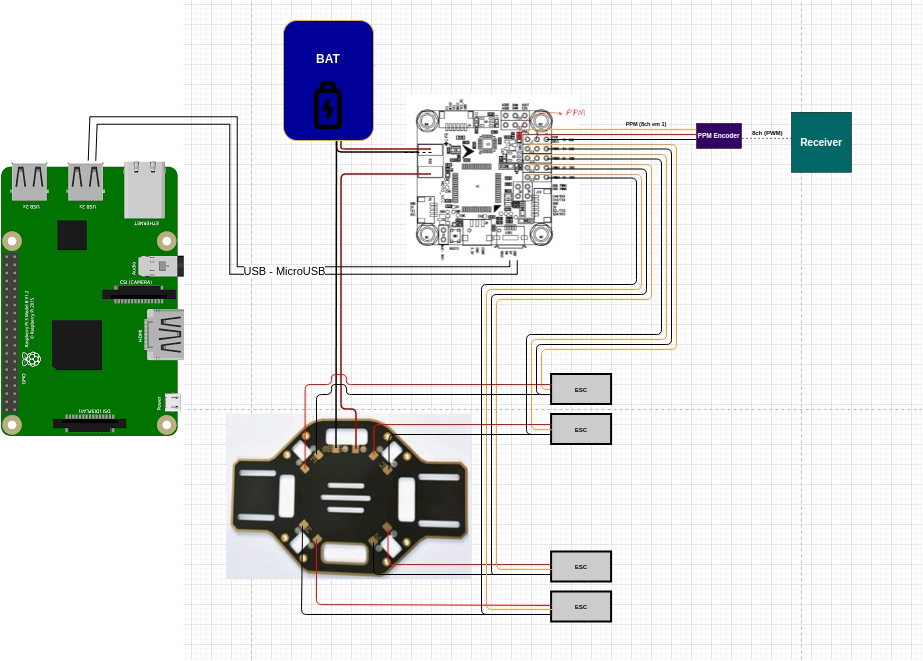
\includegraphics[width=0.7\textwidth]{Images/Diagramas/hardware_connections.png}
  \caption{Conexões de hardware para Omnibus F4 Pro V3.}
  \label{fig:hardware_connections.png.0}
\end{figure}
%
A motivação para a escolha dessa controladora foi o preço da mesma no mercado em relação às outras, valor que na época era em torno de 260 reais, enquanto que a Pixhawk custava em torno de 1000 reais. O resto dos componentes também foi escolhido com o intuito de deixar o projeto em baixo custo. 
%
\begin{figure}[!htbp]
  \centering
  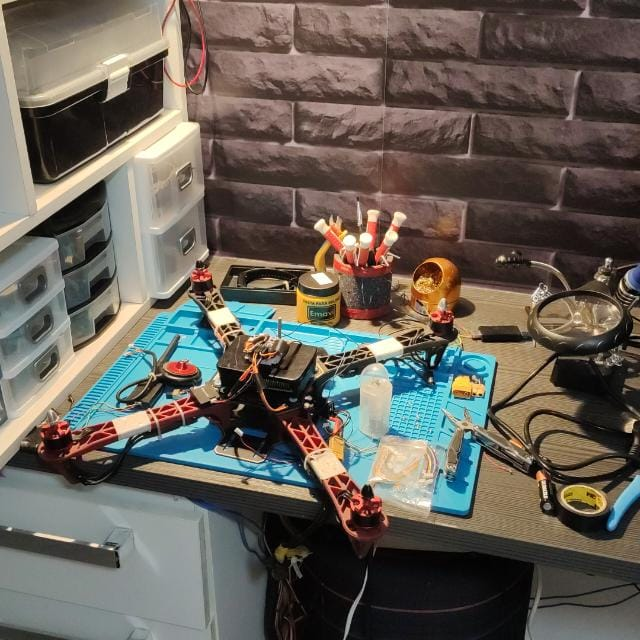
\includegraphics[width=0.7\textwidth]{Images/Desenvolvimento/omnibus_drone.jpeg}
  \caption{Bancada de trabalho com o drone quadricóptero.}
  \label{fig:omnibus_drone.jpeg.0}
\end{figure}
%

Após a ligação dos componentes eletrônicos, o teste de conexão entre o Raspberry e a controladora foi realizado utilizando o software MavProxy no minicomputador e foi possível obter dados em tempo real da controladora através da conexão serial assim como também foi possível mandar comandos MAVLink para a controladora de voo através do terminal da aplicação.

Dessa forma, conseguiu-se comandar o drone a partir do computador de bordo e receber dados de telemetria do mesmo. Entretanto, não foi possível acoplar o módulo de GPS na controladora já que o módulo em questão não se mostrou compatível com a mesma.

As pesquisas e soluções de problemas oriundos da execução dessa etapa foram cruciais para adiquirir maturidade na montagem, configuração e acoplamento dos componentes. Além disso, o conhecimento adiquirido das ferramentas utilizadas para conectar o computador de bordo ao drone também foram excenciais. Entretanto, escolhemos mudar o hardware utilizado para uma configuração de drone mais convencional na comunidade ArduPilot, com a controladora Pixhawk Cube. 

\section{Montagem do drone hexacóptero}

Após os problemas obtidos no drone quadcóptero com a controladora Omnibus, trocamos o hardware utilizado para um drone hexacóptero com a controladora Pixhawk Cube. Tal aeronave já estava operacional antes de acoplarmos o Raspberrypi, isto é, era possível realizar todas as funções básicas que a controladora por si só é capaz de fazer.
%
\begin{figure}[!htbp]
  \centering
  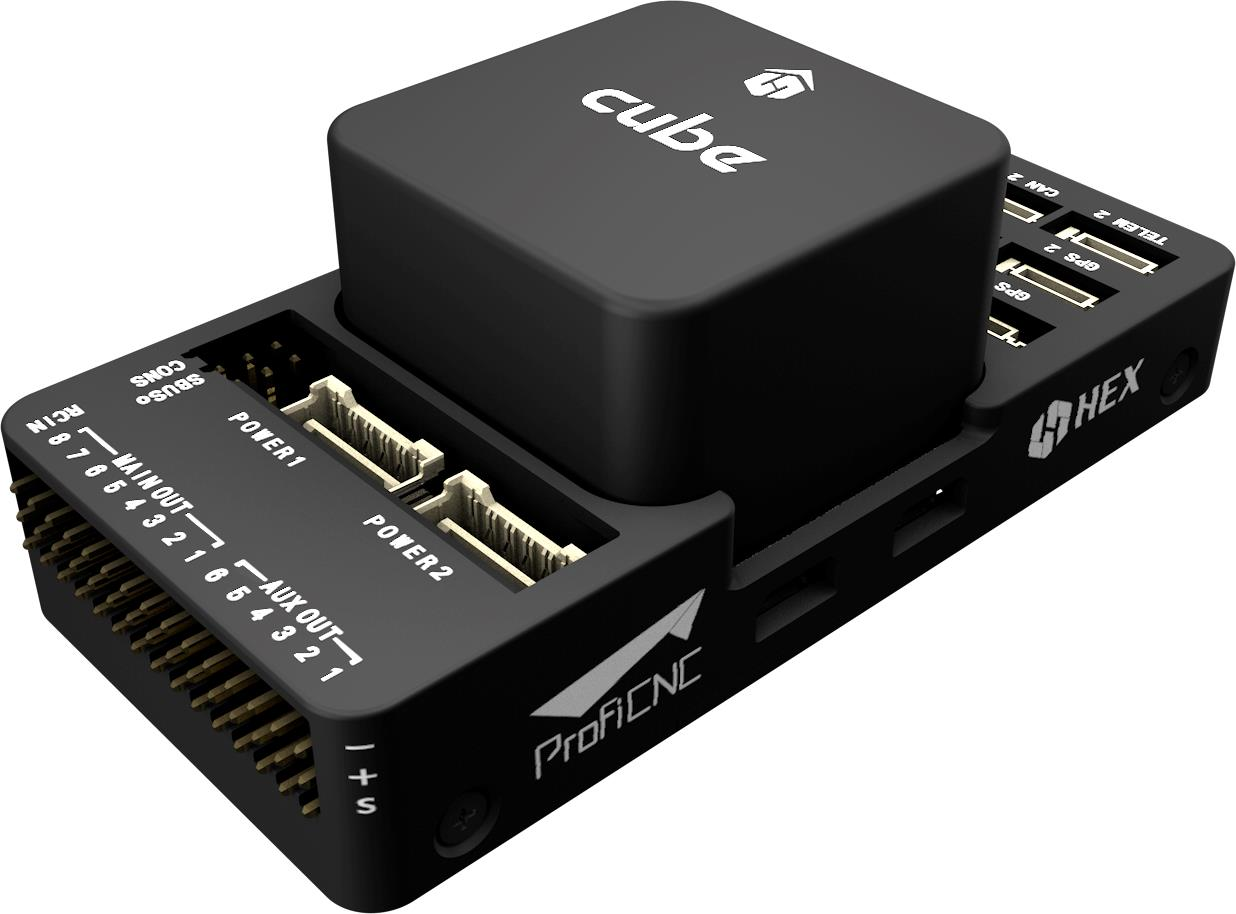
\includegraphics[width=0.4\textwidth]{Images/Desenvolvimento/pixhawk2_cube_hero.png}
  \caption{Pixhawk 2 Cube Hero.}
  \label{fig:pixhawk2_cube_hero.png.0}
\end{figure}
%

Com isso, obtemos a seguinte conexão dos componentes:

\subsection{Diagrama de conexão dos componentes de hardware}
%
\begin{figure}[!htbp]
  \centering
  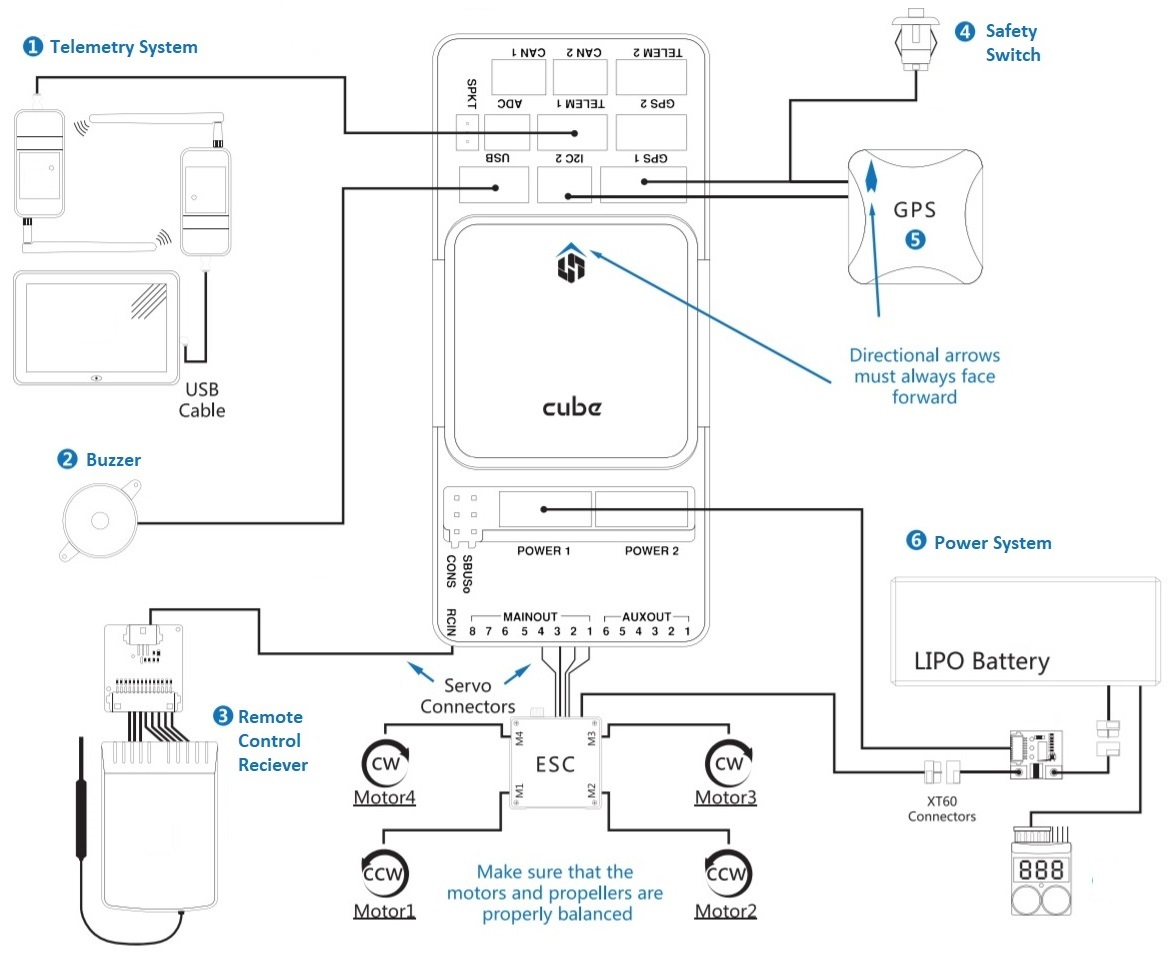
\includegraphics[width=0.7\textwidth]{Images/Diagramas/cube_wiring_overview.jpg}
  \caption{Conexões de hardware para a Pixhawk 2 Cube Hero.}
  \label{fig:cube_wiring_overview.jpg.0}
\end{figure}
%
<motivação da escolha desse hardware>
<características desse hardware>
<capacidades desse drone>
%
\begin{figure}[!htbp]
  \centering
  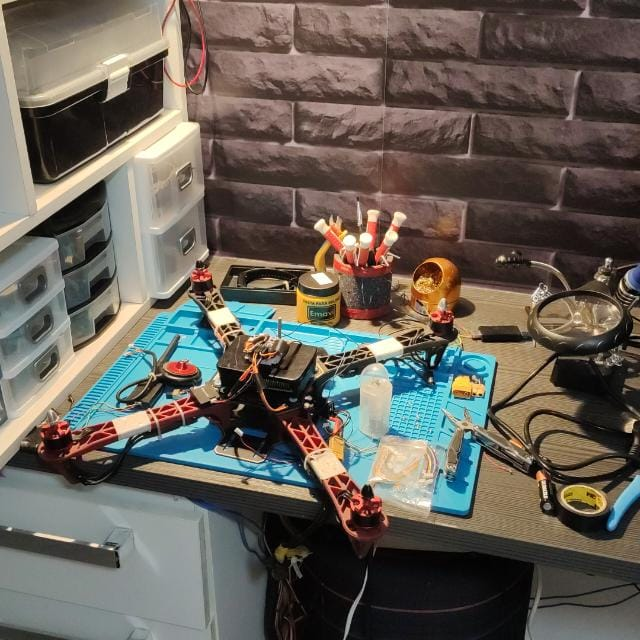
\includegraphics[width=0.7\textwidth]{Images/Desenvolvimento/omnibus_drone.jpeg}
  \caption{Bancada de trabalho com o drone quadricóptero.}
  \label{fig:omnibus_drone.jpeg.0}
\end{figure}
%
<conseguir mais fotos do drone>
<mostrar ligação dos componentes e tudo funcionando perfeitamente>
<motivação da escolha desse hardware>
<características desse hardware>
<capacidades desse drone>

\newpage

\chapter{Resultados}
%
% retira numeracao da pagina, conforme as normas de apresentacao.
\thispagestyle{empty} 
%
apresentação de resultados (numéricos e/ou gráficos) 
de cálculos e/ou de simulações, requeridos na especificação do trabalho.

%%%%%%%%%%%%%%%%%%%%%%%%%%%%%%%%%%%%%%%%%%%%%%%%%%%


%%%%%%%%%%%%%%%%%%%%%%%%%%%%%%%%%%%%%%%%%%%%%%%%%%%%%%%%
%                      Conclusão                       %
%%%%%%%%%%%%%%%%%%%%%%%%%%%%%%%%%%%%%%%%%%%%%%%%%%%%%%%%

\chapter{Conclusão}
%
% retira numeracao da pagina, conforme as normas de apresentacao.
\thispagestyle{empty} 
%

\hl{Hipótese testada
Se realizarmos o experimento em outro ambiente com maior capacidade para que todos possam assistir de forma homogênea atenderemos a demanda da turma, teremos um aprendizado mais efetivo e melhoria no tempo dedicado a esse experimento.

Responda as perguntas avaliativas para definir a conclusão}
\begin{enumerate}
    \item Com o sistema desenvolvido será possível ao professor usuário controlar o experimento proposto remotamente?
    \item pergunta avaliativa 2
    \item pergunta avaliativa 3
    \item pergunta avaliativa 4
\end{enumerate}

Esta monografia tem como base a pesquisa, a elaboração e o teste, em ambiente simulado, de um drone capaz de se comunicar por uma rede IP, no nosso caso,
uma rede \textit{wi-fi}. 

Aproveitou-se conhecimentos adquiridos na equipe UFFO \cite{url:equipeuffo}, como \textit{softwares} e bibliotecas específicas para automação. A partir
dessa base, surgiu a ideia de incrementar o \textit{hardware} de um drone comum acoplando um \textit{raspberry}. A grande adição é o acesso ao protocolo IP, permitindo o drone trocar dados sem limitações de distância. Para realizar a comunicação com o drone, foi elaborada uma arquitetura de cliente-servidor, cujo cliente, em resumo o drone, envia e recebe dados do servidor, ambos conectados numa mesma rede, via VPN. Por fim, realizou-se uma página \textit{web} como \textit{interface} gráfica final, a qual permite o envio de missões ao drone e exibe os dados essenciais de telemetria em tempo real.  

No geral, os resultados foram compatíveis aos objetivos propostos, realizaram-se testes no ambiente de simulação que demonstraram a viabilidade de um projeto prático.  

O projeto como um todo ainda deve ser aperfeiçoado casa haja interesse em comercialização. Faz-se necessário a realização de testes com um drone fora do ambiente de simulação, e como citado no Capítulo 1~\ref{item:solucao}, idealmente, conectar um modem LTE ou NR ao \textit{raspberry}. Ambos, os testes e a conexão do modem, podem ser feitos por futuros integrantes da equipe UFFO.


%%%%%%%%%%%%%%%%%%%%%%%%%%%%%%%%%%%%%%%%%%%%%%%%%%%%%%%%
%          Sugestoes para trabalhos futuros            %
%%%%%%%%%%%%%%%%%%%%%%%%%%%%%%%%%%%%%%%%%%%%%%%%%%%%%%%%

\chapter{Sugestões para trabalhos futuros}
%
% retira numeracao da pagina, conforme as normas de apresentacao.
\thispagestyle{empty} 
%
%
Tendo em mente as características do projeto apresentadas neste trabalho, podemos imaginar diversas aplicações para serem acrescentadas. Somos capazes, portanto, de listar algumas das possíveis aplicações e seus possíveis desdobramentos.
%
\begin{enumerate}
    \item Melhorias na interface de controle 
        \begin{enumerate}
            \item Adição de novos funcionalidades
            \item Coleta e apresentação de mais dados do drone  
        \end{enumerate}
    \item Integração de um modem de internet móvel
        \begin{enumerate}
            \item Controle e coleta de dados a qualquer distância, desde que haja sinal de internet móvel.
        \end{enumerate}
    \item Integração de uma câmera
        \begin{enumerate}
            \item Visão em tempo real do ambiente o qual o drone sobrevoa
            \item Adição de inteligência artificial capaz de tratar e processar imagens capturadas
        \end{enumerate}
\end{enumerate}

Para cada uma dessas adições deve-se realizar testes de viabilidade, bem como estudos mais profundos do impacto que cada complemento teria no modelo final deste trabalho. 

Portanto, geradas essas necessidades, podemos utilizar o ambiente de simulação do gazebo, junto aos módulos ROS, para prever como se comportará o sistema. Comparações a respeito do desempenho geral podem e devem ser feitas a fim de comprovar bons resultados.

%%%%%%%%%%%%%%%%%%%%%%%%%%%%%%%%%%%%%%%%%%%%%%%%%%%%%%


%%%%%%%%%%%%%%%%%%%%%%%%%%%%%%%%%%%%%%%%%%%%%%%%%%%%%%%%%%%%%%%%%%%
%                  Referencias Bibliograficas                     % 
%%%%%%%%%%%%%%%%%%%%%%%%%%%%%%%%%%%%%%%%%%%%%%%%%%%%%%%%%%%%%%%%%%%

\bibliographystyle{apalike}
%
\bibliography{./MyBibFiles/my_refs}
%
\addcontentsline{toc}{chapter}{\refname}
%
\thispagestyle{myheadings}

%
%%%%%%%%%%%%%%%%%%%%%%%%%%%%%%%%%%%%%%%%%%%%%%%%%%%%

%
%%%%%%%%%%%%%%%%%%%%%%%%%%%%%%%%%%%%%%%%%%%%%%%%
%
%
% Apendices e anexos
%
\appendix
%
%
%%%%%%%%%%%%%%%%%%%%%%%%%%%%%%%%%%%%%%%%%%%%%%%%%%%%%%%%
%
\chapter{Apêndice 1}
%
% retira numeracao da pagina, conforme as normas de apresentacao.
\thispagestyle{empty} 
%
Segue abaixo um guia de instalação completo dos \textit{Softwares} de simulação e suas respectivas dependências para Ubuntu 20.04 LTS.

\section{Intalando o ArduPilot e MavProxy}

\subsection{Clonando o repositório \textit{git} para sua máquina}
\begin{lstlisting}[language=bash]
  $ cd ~
  $ sudo apt install git
  $ git clone https://github.com/ArduPilot/ardupilot.git
\end{lstlisting}

\subsection{Instalando as dependências e recompilando o perfil}
\begin{lstlisting}[language=bash]
  $ cd ardupilot/Tools/environment_install/install-prereqs-ubuntu.sh -y
  $ . ~/.profile
\end{lstlisting}

\subsection{Mudando para a \textit{branch} do ArduCopter}
\begin{lstlisting}[language=bash]
  $ git checkout Copter-4.0.4
  $ git submodule update --init --recursive
\end{lstlisting}

\subsection{Rodando SITL (\textit{Software In The Loop})}
\begin{lstlisting}[language=bash]
  $ cd ~/ardupilot/ArduCopter
  $ sim_vehicle.py -w
\end{lstlisting}

\section{Instalando o Gazebo e o \textit{plugin} do ArduPilot}

\subsection{Atualizando a lista de fontes para \textit{download}}
\begin{lstlisting}[language=bash]
  $ sudo sh -c 'echo "deb http://packages.osrfoundation.org/gazebo/ubuntu-stable `lsb_release -cs` main" > /etc/apt/sources.list.d/gazebo-stable.list'
  $ wget http://packages.osrfoundation.org/gazebo.key -O - | sudo apt-key add -
  $ sudo apt update
\end{lstlisting}

\subsection{Instalando o \textit{plugin} do Gazebo para comunicação com o ArduPilot}
\begin{lstlisting}[language=bash]
  $ cd ~
  $ git clone https://github.com/khancyr/ardupilot_gazebo.git
  $ cd ardupilot_gazebo
  $ mkdir build
  $ cd build
  $ cmake ..
  $ make -j4
  $ sudo make install
  $ echo 'source /usr/share/gazebo/setup.sh' >> ~/.bashrc
  $ echo 'export GAZEBO_MODEL_PATH=~/ardupilot_gazebo/models' >> ~/.bashrc
  $ . ~/.bashrc
\end{lstlisting}

\subsection{Executando a simulação}
\begin{lstlisting}[language=bash]
  No primeiro terminal do linux rode o Gazebo: 
  $ gazebo --verbose ~/ardupilot_gazebo/worlds/iris_arducopter_runway.world
  
  No segundo terminal do linux rode o SITL:
  $ cd ~/ardupilot/ArduCopter/
  $ sim_vehicle.py -v ArduCopter -f gazebo-iris --console
\end{lstlisting}

\section{Instalando o \textit{ROS} e o configurando o \textit{Catkin}}

\subsection{Atualizando a lista de fontes para \textit{download}}
\begin{lstlisting}[language=bash] 
  $ sudo sh -c 'echo "deb http://packages.ros.org/ros/ubuntu $(lsb_release -sc) main" > /etc/apt/sources.list.d/ros-latest.list'
  $ sudo apt install curl
  $ curl -s https://raw.githubusercontent.com/ros/rosdistro/master/ros.asc | sudo apt-key add -
  $ sudo apt update
\end{lstlisting}

\subsection{Instalando o \textit{ROS}}
\begin{lstlisting}[language=bash] 
  $ sudo apt install ros-noetic-desktop-full
\end{lstlisting}

\subsection{Configurando o ambiente}
\begin{lstlisting}[language=bash] 
  $ source /opt/ros/noetic/setup.bash
  $ echo "source /opt/ros/noetic/setup.bash" >> ~/.bashrc
  $ source ~/.bashrc
  $ echo "source /opt/ros/noetic/setup.zsh" >> ~/.zshrc
  $ source ~/.zshrc
\end{lstlisting}

\subsection{Instalando as dependências para os pacotes dos \textit{ROS}}
\begin{lstlisting}[language=bash] 
  $ sudo apt install python3-rosdep python3-rosinstall python3-rosinstall-generator python3-wstool build-essential
  $ sudo apt install python3-rosdep
  $ sudo rosdep init
  $ rosdep update
\end{lstlisting}

\subsection{Configurando o \textit{Catkin}}
\begin{lstlisting}[language=bash] 
  $ sudo apt-get install python3-wstool python3-rosinstall-generator python3-catkin-lint python3-pip python3-catkin-tools
  $ pip3 install osrf-pycommon
  $ mkdir -p ~/catkin_ws/src
  $ cd ~/catkin_ws
  $ catkin init
\end{lstlisting}

\subsection{Instalando as dependências para o \textit{Catkin}}
\begin{lstlisting}[language=bash] 
  $ sudo apt-get install python3-wstool python3-rosinstall-generator python3-catkin-lint python3-pip python3-catkin-tools
  $ pip3 install osrf-pycommon
  $ mkdir -p ~/catkin_ws/src
  $ cd ~/catkin_ws
  $ catkin init
\end{lstlisting}

\subsection{Instalando as \textit{MAVROS} e \textit{MAVLink}}
\begin{lstlisting}[language=bash] 
  $ cd ~/catkin_ws
  $ wstool init ~/catkin_ws/src
  $ rosinstall_generator --upstream mavros | tee /tmp/mavros.rosinstall
  $ rosinstall_generator mavlink | tee -a /tmp/mavros.rosinstall
  $ wstool merge -t src /tmp/mavros.rosinstall
  $ wstool update -t src
  $ rosdep install --from-paths src --ignore-src --rosdistro `echo $ROS_DISTRO' -y
  $ catkin build
\end{lstlisting}

\subsection{Atualizando o arquivo \textit{.bachrc}}
\begin{lstlisting}[language=bash] 
  $ echo "source ~/catkin_ws/devel/setup.bash" >> ~/.bashrc
  $ source ~/.bashrc
\end{lstlisting}

\section{Instalando as dependências geográficas e clonando o repositório de simulação do \textit{Intelligent Quads}}

\subsection{Instalando as dependências geográficas}
\begin{lstlisting}[language=bash] 
  $ sudo ~/catkin_ws/src/mavros/mavros/scripts/install_geographiclib_datasets.sh]
\end{lstlisting}

\subsection{Clonando pacote ROS de simulação do \textit{Intelligent Quads}}
\begin{lstlisting}[language=bash] 
  $ cd ~/catkin_ws/src
  $ git clone https://github.com/Intelligent-Quads/iq_sim.git
  $echo "GAZEBO_MODEL_PATH=${GAZEBO_MODEL_PATH}:$HOME/catkin_ws/src/iq_sim/models" >> ~/.bashrc
  $ cd ~/catkin_ws
  $ catkin build
  $ source ~/.bashrc
\end{lstlisting}

\section{Instalando o \textit{QGround Control}}

\subsection{Alterando permissões e instalando o \textit{QGround Control}}
\begin{lstlisting}[language=bash] 
  $ sudo usermod -a -G dialout $USER
  $ sudo apt-get remove modemmanager
  $ wget https://s3-us-west-2.amazonaws.com/qgroundcontrol/latest/QGroundControl.AppImage
  $ chmod +x ./QGroundControl.AppImage 
  $ ./QGroundControl.AppImage
\end{lstlisting}
%
%%%%%%%%%%%%%%%%%%%%%%%%%%%%%%%%%%%%%%%%%%%%%%%%%%%%%%%%
%
\end{document}
%


%%%%%%%%%%%%%%%%%%%%%%%%%%%%%%%%%%%%%%%%
%     Insercao do Indice Remissivo     %
%%%%%%%%%%%%%%%%%%%%%%%%%%%%%%%%%%%%%%%%
%
% Makeindex Database 
% (baseada nos arquivos: XXX.idx --> xxx.ind --> xxx.ilg)
%
\printindex
%
\addcontentsline{toc}{chapter}{\indexname}
%
\thispagestyle{myheadings}


%%%%%%%%%%%%%%%%%%%%%%%%%%%%%%%%%%%%%%%%%%%%%%%%%%%%%%


%
\end{document}
%

%%%%%%%%%%%%%%%%%
% Fim do modelo %
%%%%%%%%%%%%%%%%%
